\documentclass[compress]{beamer}
\usepackage{ifthen}

\title{Preview of MC and MTCC track-based Alignments \\ and observation of MTCC Noise}
\author{Jim Pivarski, Alexei Safonov}
\institute{Texas A\&M University}
\date{ 7 June, 2007}

\setbeamertemplate{navigation symbols}{}
\setbeamertemplate{headline}{\includegraphics[height=1 cm]{../cmslogo} \hspace{0.1 cm} \includegraphics[height=1 cm]{../tamulogo} \hfill
\begin{minipage}{9 cm}
\vspace{-0.75 cm} \small
\begin{center}
\ifthenelse{\equal{\insertpagenumber}{1}}{}{\insertsection}
\end{center}
\end{minipage} \hfill
\begin{minipage}{1 cm}
\vspace{-0.75 cm} \small
\begin{center}
\ifthenelse{\equal{\insertpagenumber}{1}}{}{\insertpagenumber/\pageref{numpages}}
\end{center}
\end{minipage}}

%% \xdefinecolor{verylightgray}{rgb}{0.95,0.95,0.95}
%% \beamertemplateshadingbackground{verylightgray}{white}

\begin{document}
\frame{\titlepage}
\section*{MC/MTCC Alignments and MTCC Noise --- Jim Pivarski}

\begin{frame}
\frametitle{Ongoing Activities}
\begin{itemize}\setlength{\itemsep}{0.5 cm}
\item Testing HIP alignment procedure on 26k- and 260k-event
  $Z\to\mu\mu$ MC samples to debug and optimize the procedure

\begin{itemize}\setlength{\itemsep}{0.2 cm}
\item Equivalent to 10 pb$^{-1}$ and 100 pb$^{-1}$ of $Z+W$ muons

\item Will extrapolate to low-energy muons using $J/\psi$ residuals

\item New in this test:
\begin{itemize}
\item random misalignments (1 mm RMS)
\item more ambitious precision goals (200 $\mu$m, rather than 1 cm)
\item fitting and aligning the same hits (e.g. standAloneMuons)
\end{itemize}
\end{itemize}

\item Real alignment on MTCC data (with Karoly)

\begin{itemize}\setlength{\itemsep}{0.2 cm}
\item Chamber-by-chamber and layer-by-layer

\item We expect $\sim$mm precision with this one-run test sample

\item (Re-?)Discovered wire noise in ME+1/3

\end{itemize}
\end{itemize}
\end{frame}

\begin{frame}
\frametitle{MC status: poor convergence}

\begin{columns}
\column{0.5\linewidth}
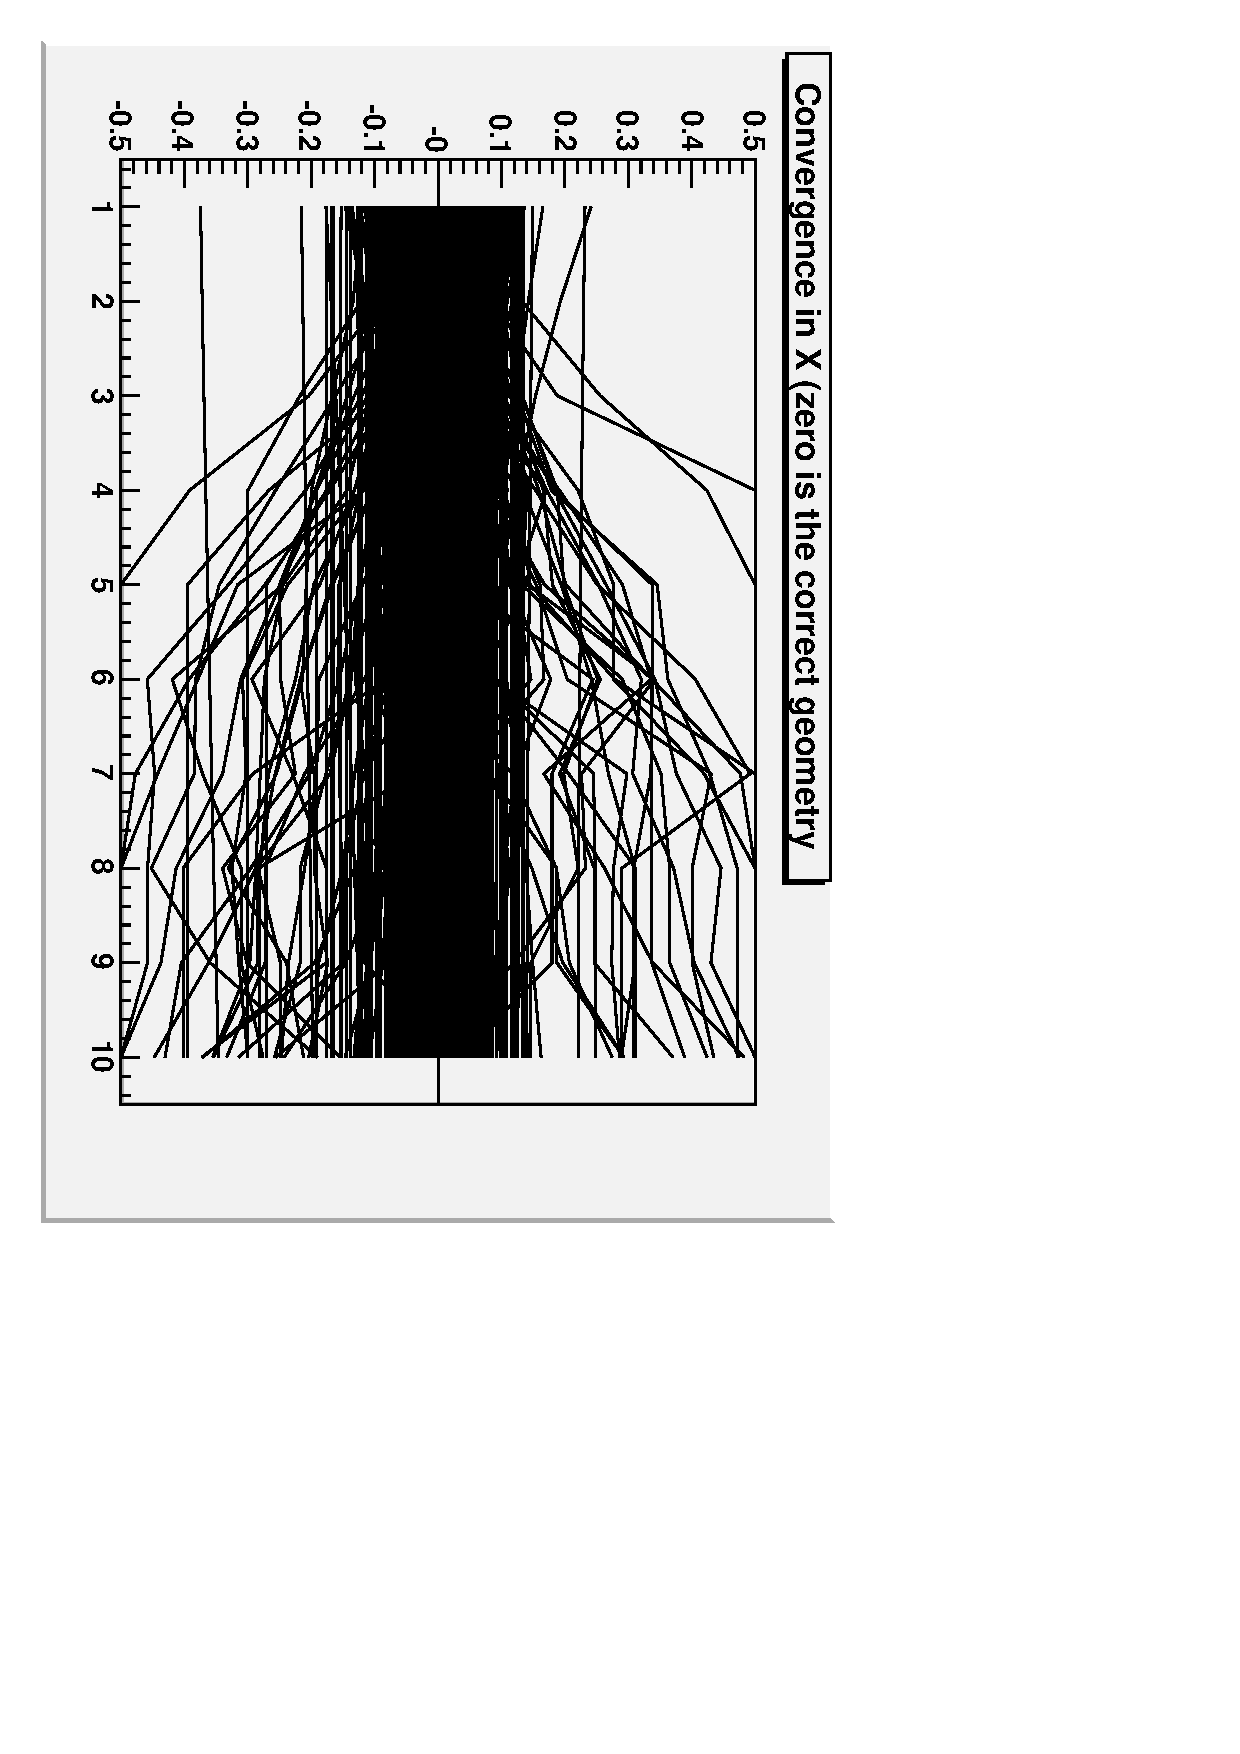
\includegraphics[height=\linewidth, angle=90]{csc_lack_of_convergence.pdf}
\column{0.5\linewidth}
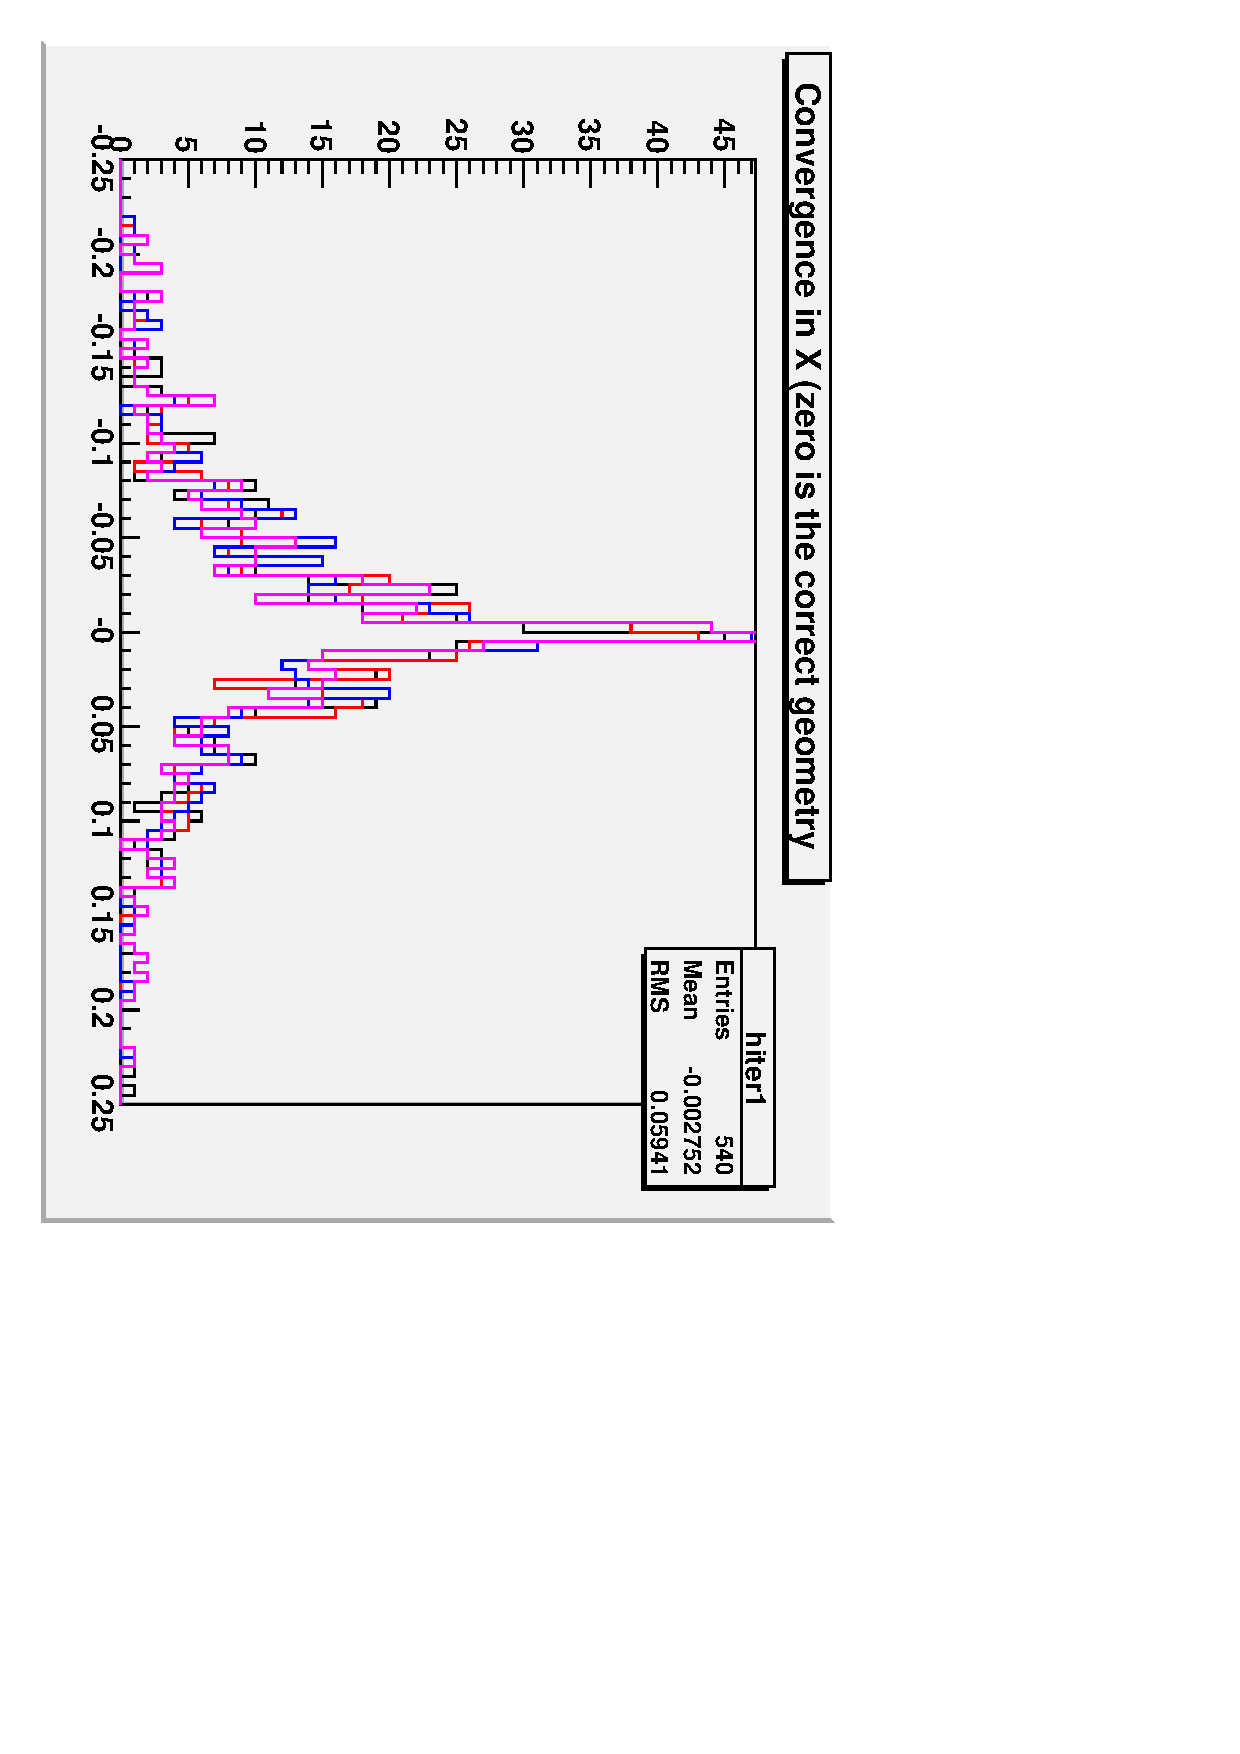
\includegraphics[height=\linewidth, angle=90]{csc_lack_of_convergence_hist.pdf}
\end{columns}

\vfill
\begin{itemize}
\item Above are CSCs, units are centimeters

\item Same behavior observed in standAlone and globalMuons

\item But unbiased tracker-to-muon sample converged (see talk at UCLA
  EMU meeting): problem is related to track-fitting bias?
\end{itemize}
\end{frame}

\begin{frame}
\frametitle{Double-peak structure in residuals}
\begin{tabular}{p{0.65\linewidth} c p{0.3\linewidth}}
\begin{minipage}{\linewidth}
  \vspace{-0.25 cm}
  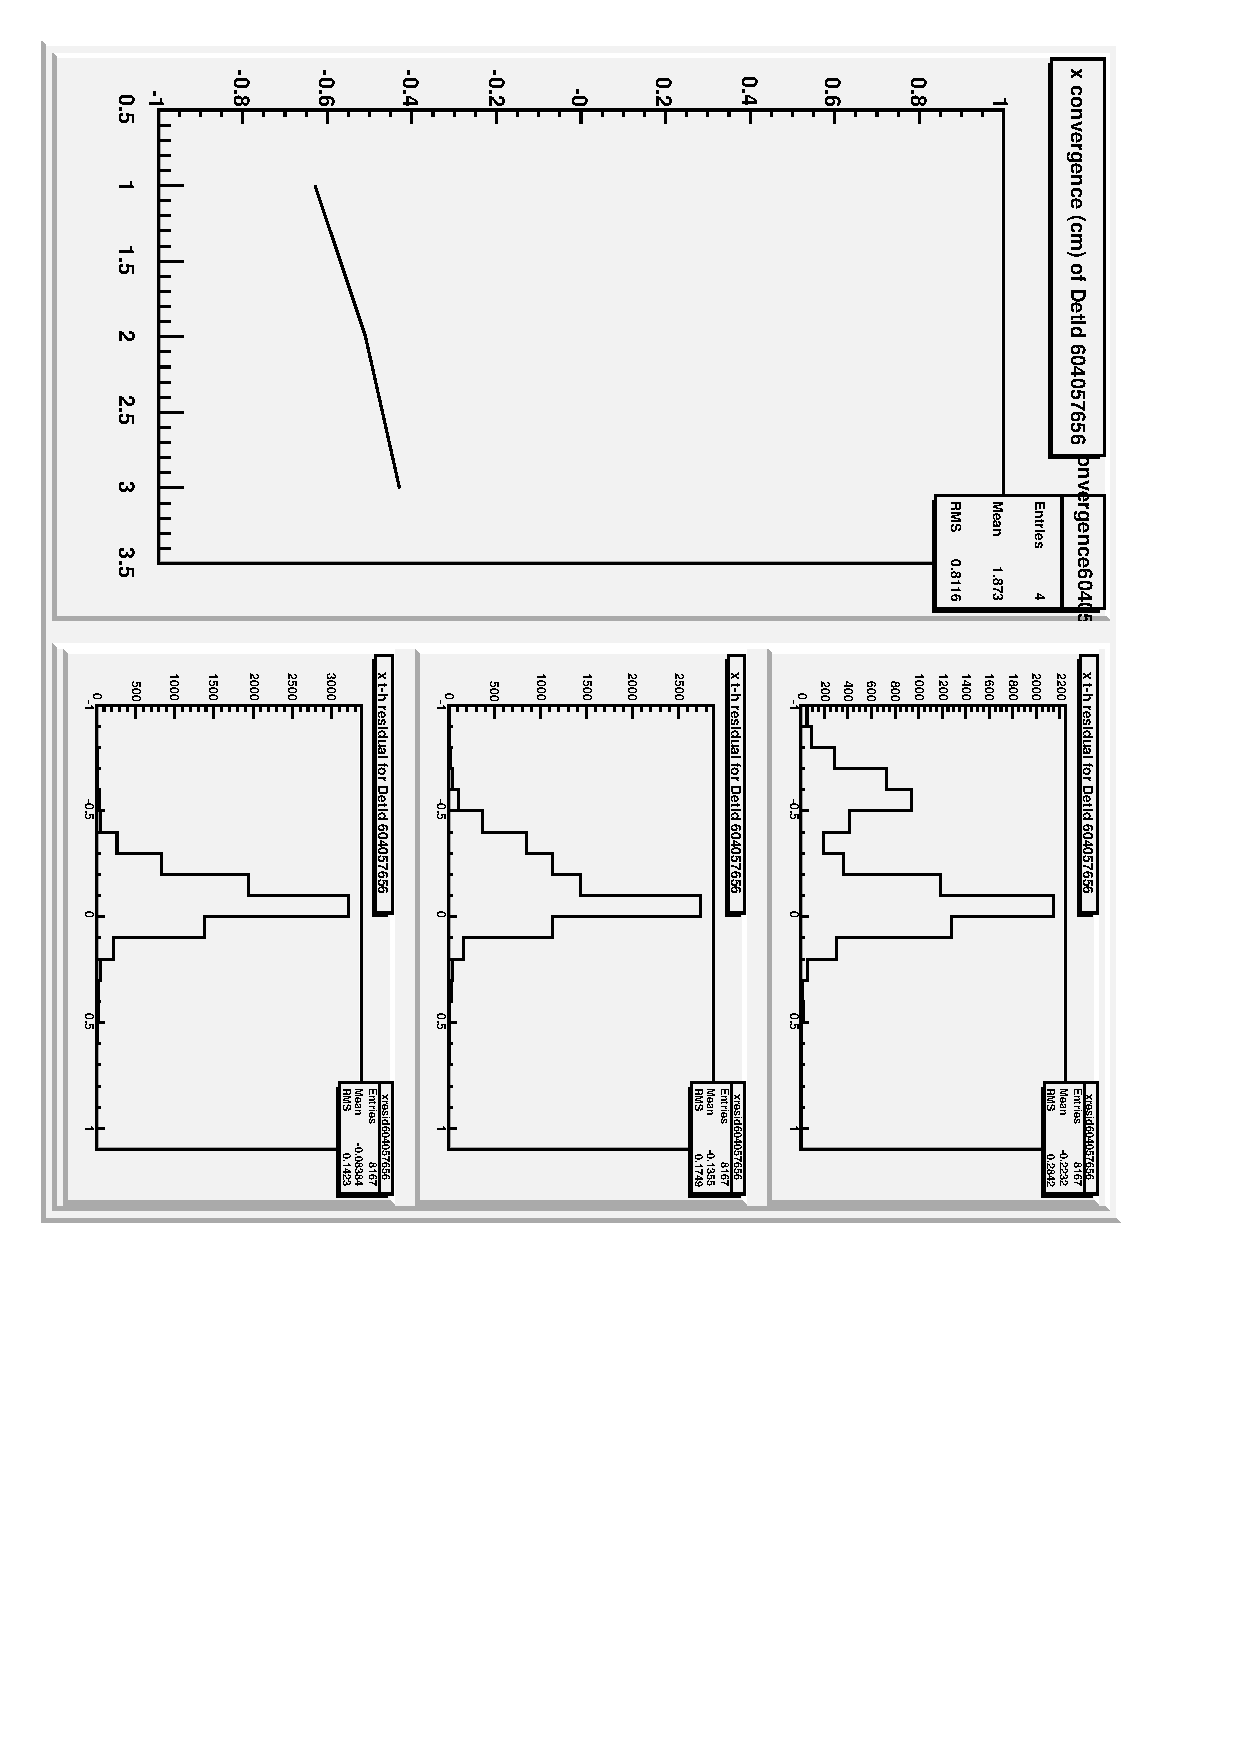
\includegraphics[height=\linewidth, angle=90]{sometimes-trusted_chamber2.pdf}

  \vspace{0.25 cm} \mbox{ }
\end{minipage} & &
\begin{minipage}{\linewidth}
  \vspace{-0.5 cm}
  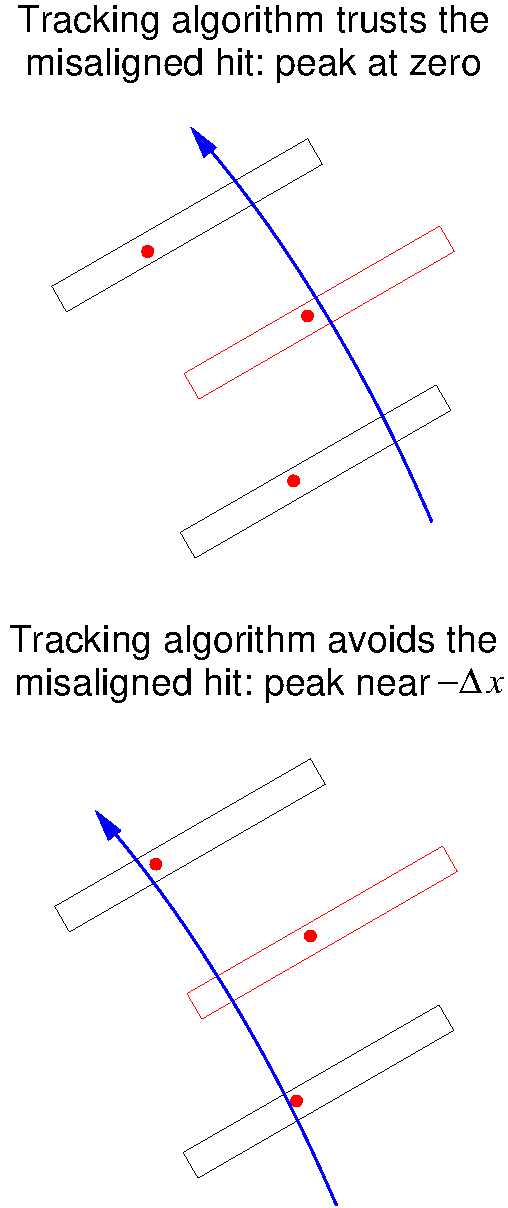
\includegraphics[width=\linewidth]{two_cases.pdf}

  \vspace{0.5 cm} \mbox{ }
\end{minipage}
\end{tabular}
\end{frame}

\begin{frame}
\frametitle{Test by misaligning all chambers $\Delta x = -1$ cm}
\begin{center}
\begin{tabular}{p{0.4\linewidth} c p{0.4\linewidth}}
  \begin{minipage}{\linewidth}
    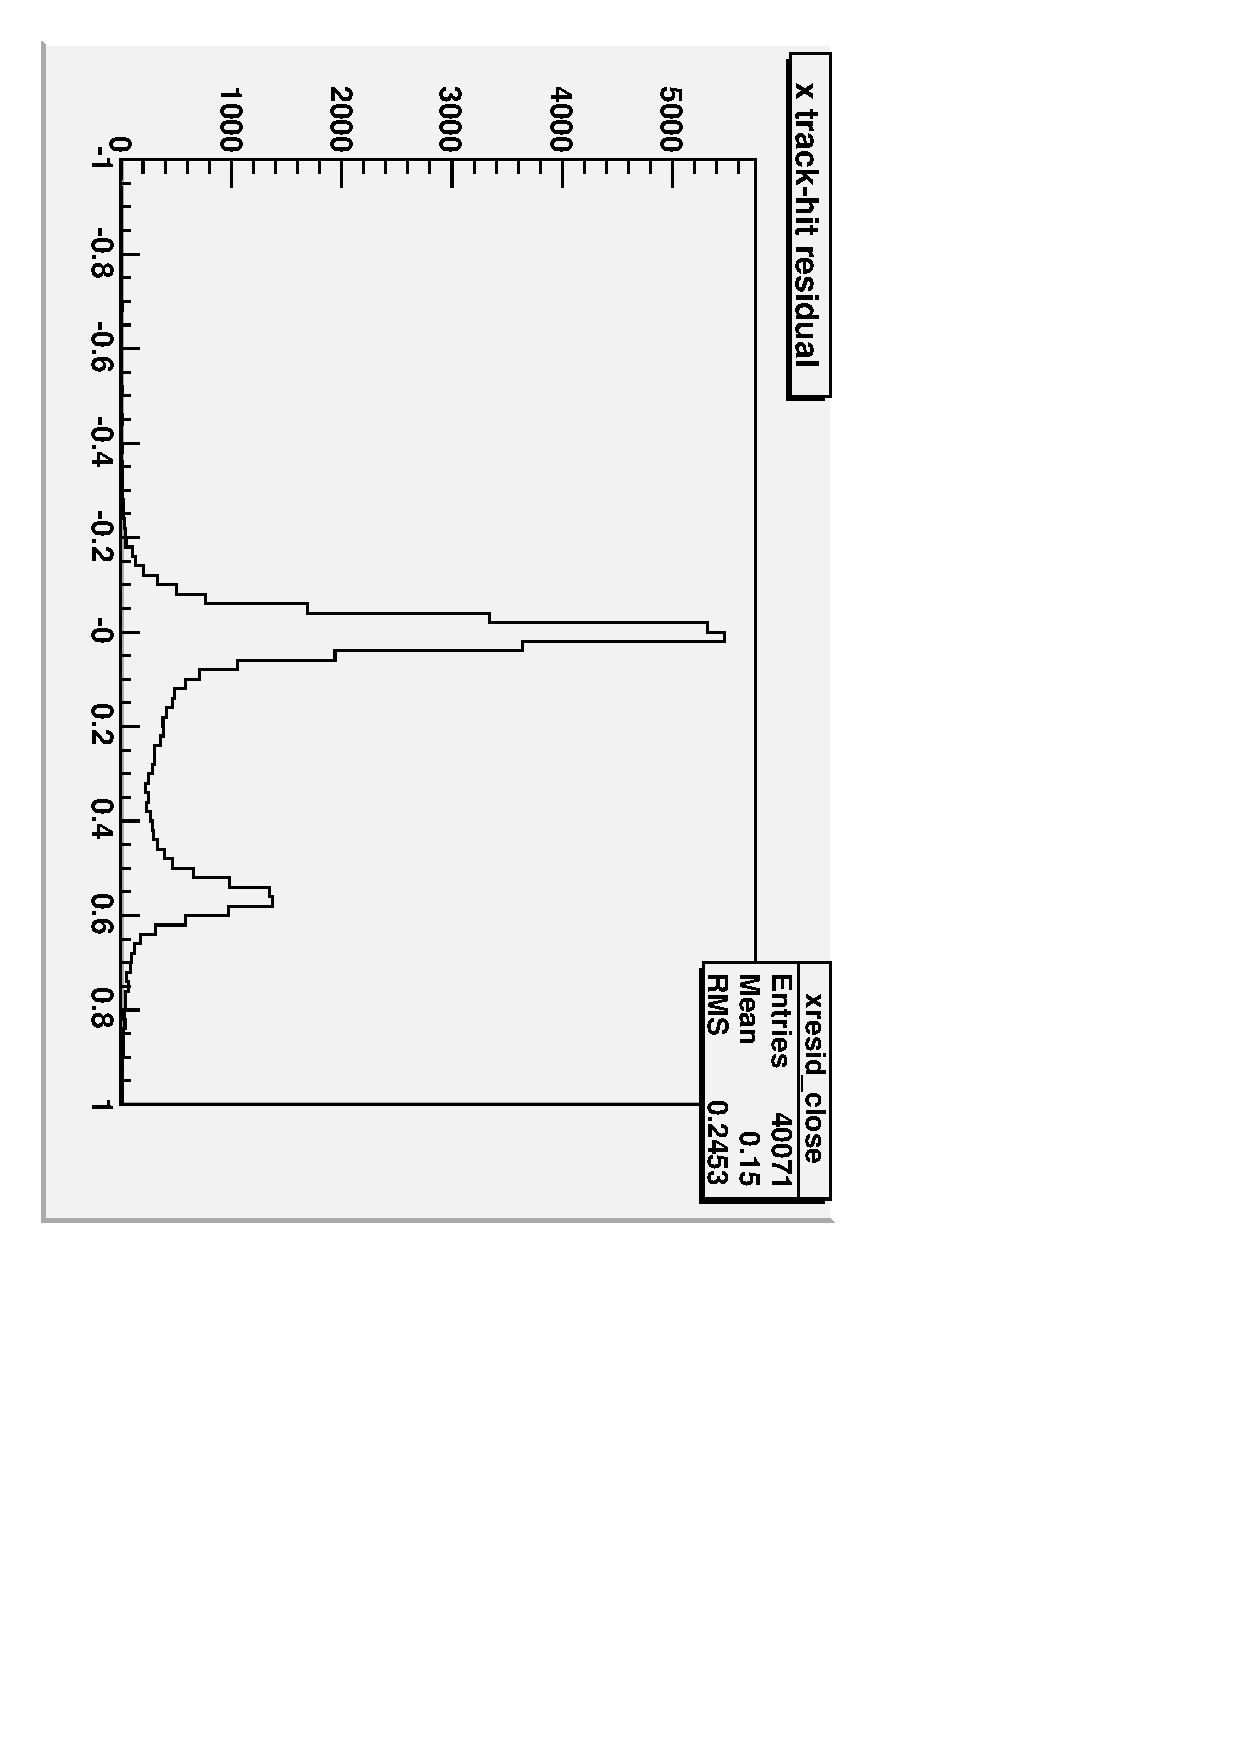
\includegraphics[height=\linewidth, angle=90]{globalMuon_x1cm_residuals.pdf}
  \end{minipage} & &
  \begin{minipage}{\linewidth}
    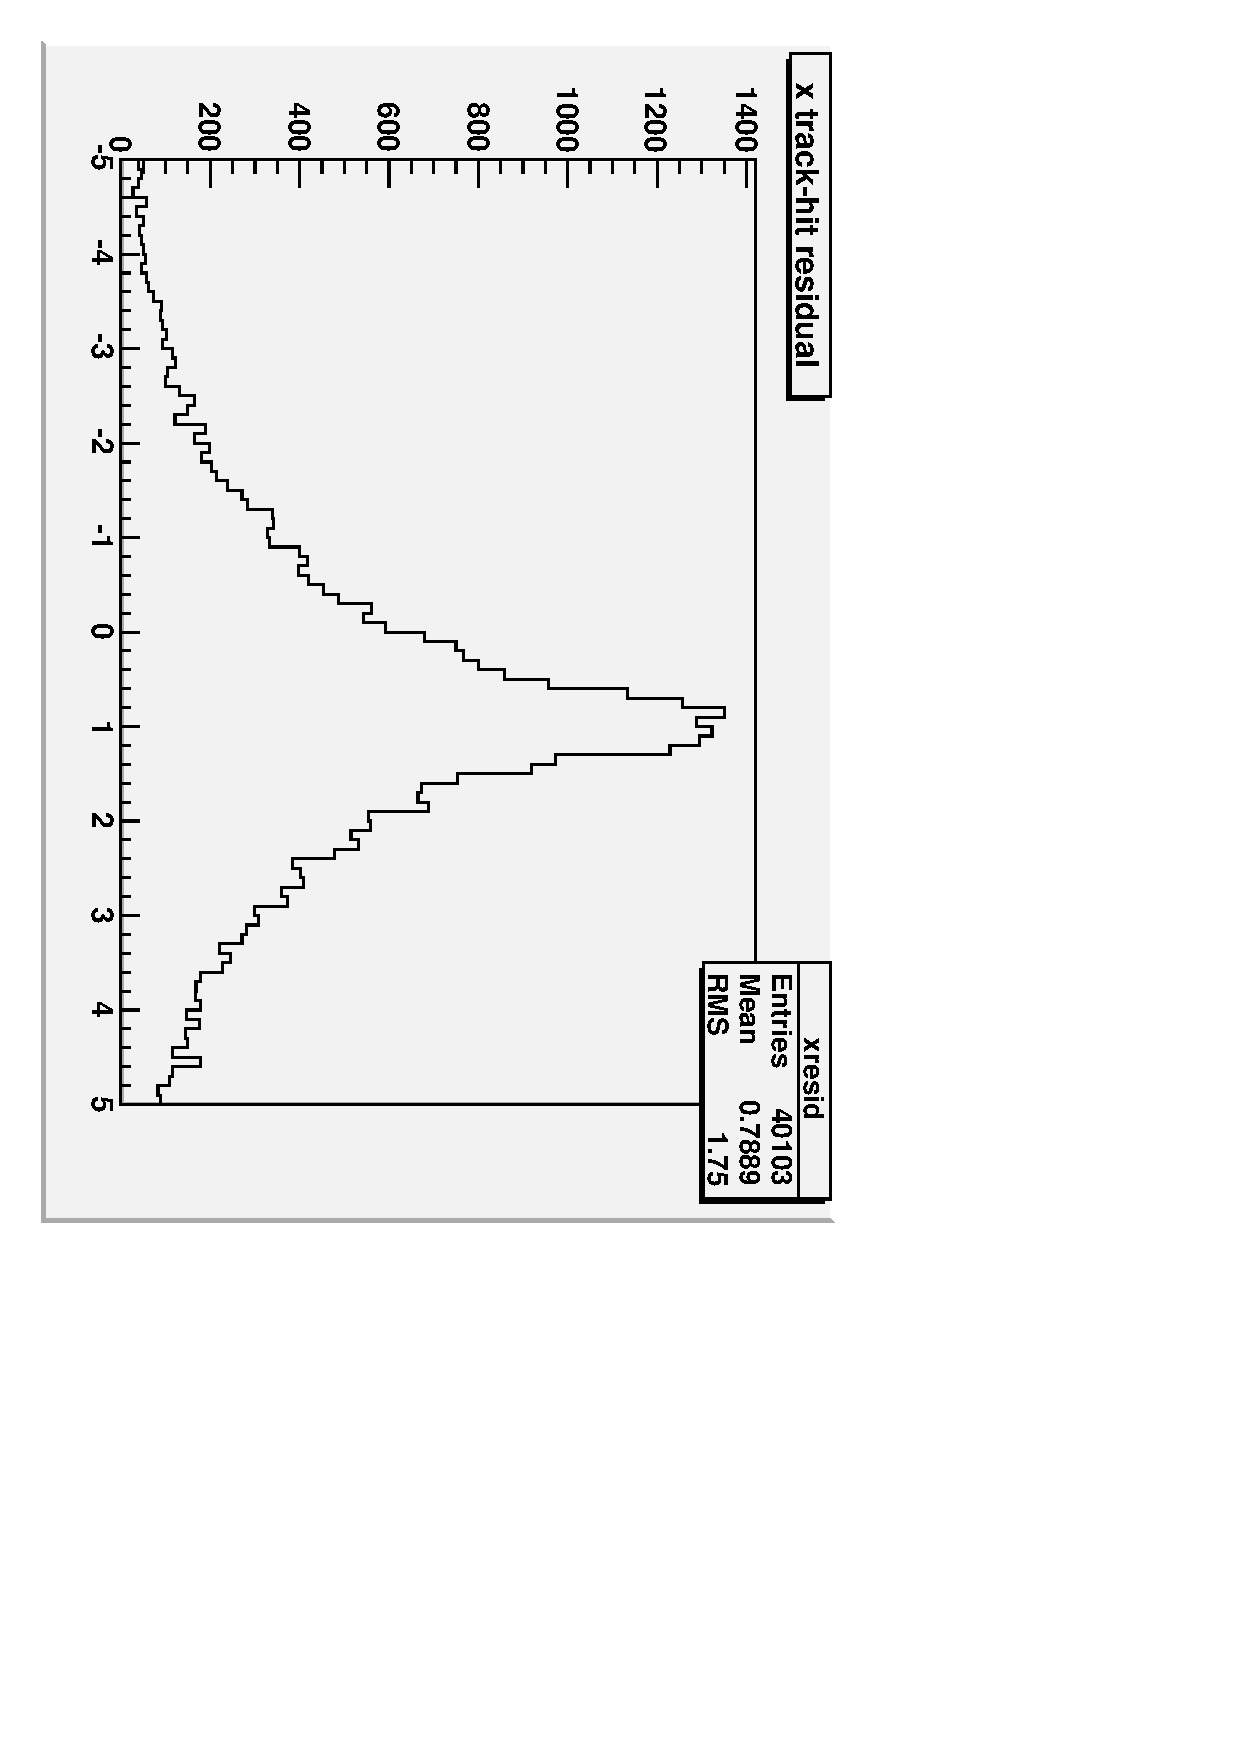
\includegraphics[height=\linewidth, angle=90]{trackerToMuon_x1cm_residuals_wide.pdf}
  \end{minipage} \\
  \begin{minipage}{\linewidth}
    \begin{center}
      globalMuons residuals
    \end{center}
  \end{minipage} & &
  \begin{minipage}{\linewidth}
    \begin{center}
      ``tracker-to-muons''
    \end{center}
  \end{minipage} \\
  & & \\
  \begin{minipage}{\linewidth}
    \begin{center}
      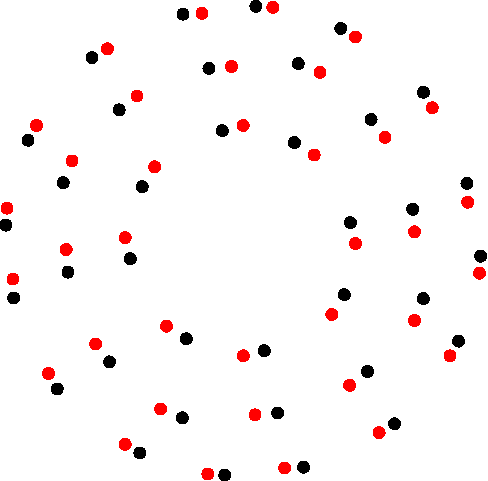
\includegraphics[width=0.6\linewidth]{wheel.pdf}
    \end{center}
  \end{minipage} & &
  \begin{minipage}{\linewidth}
    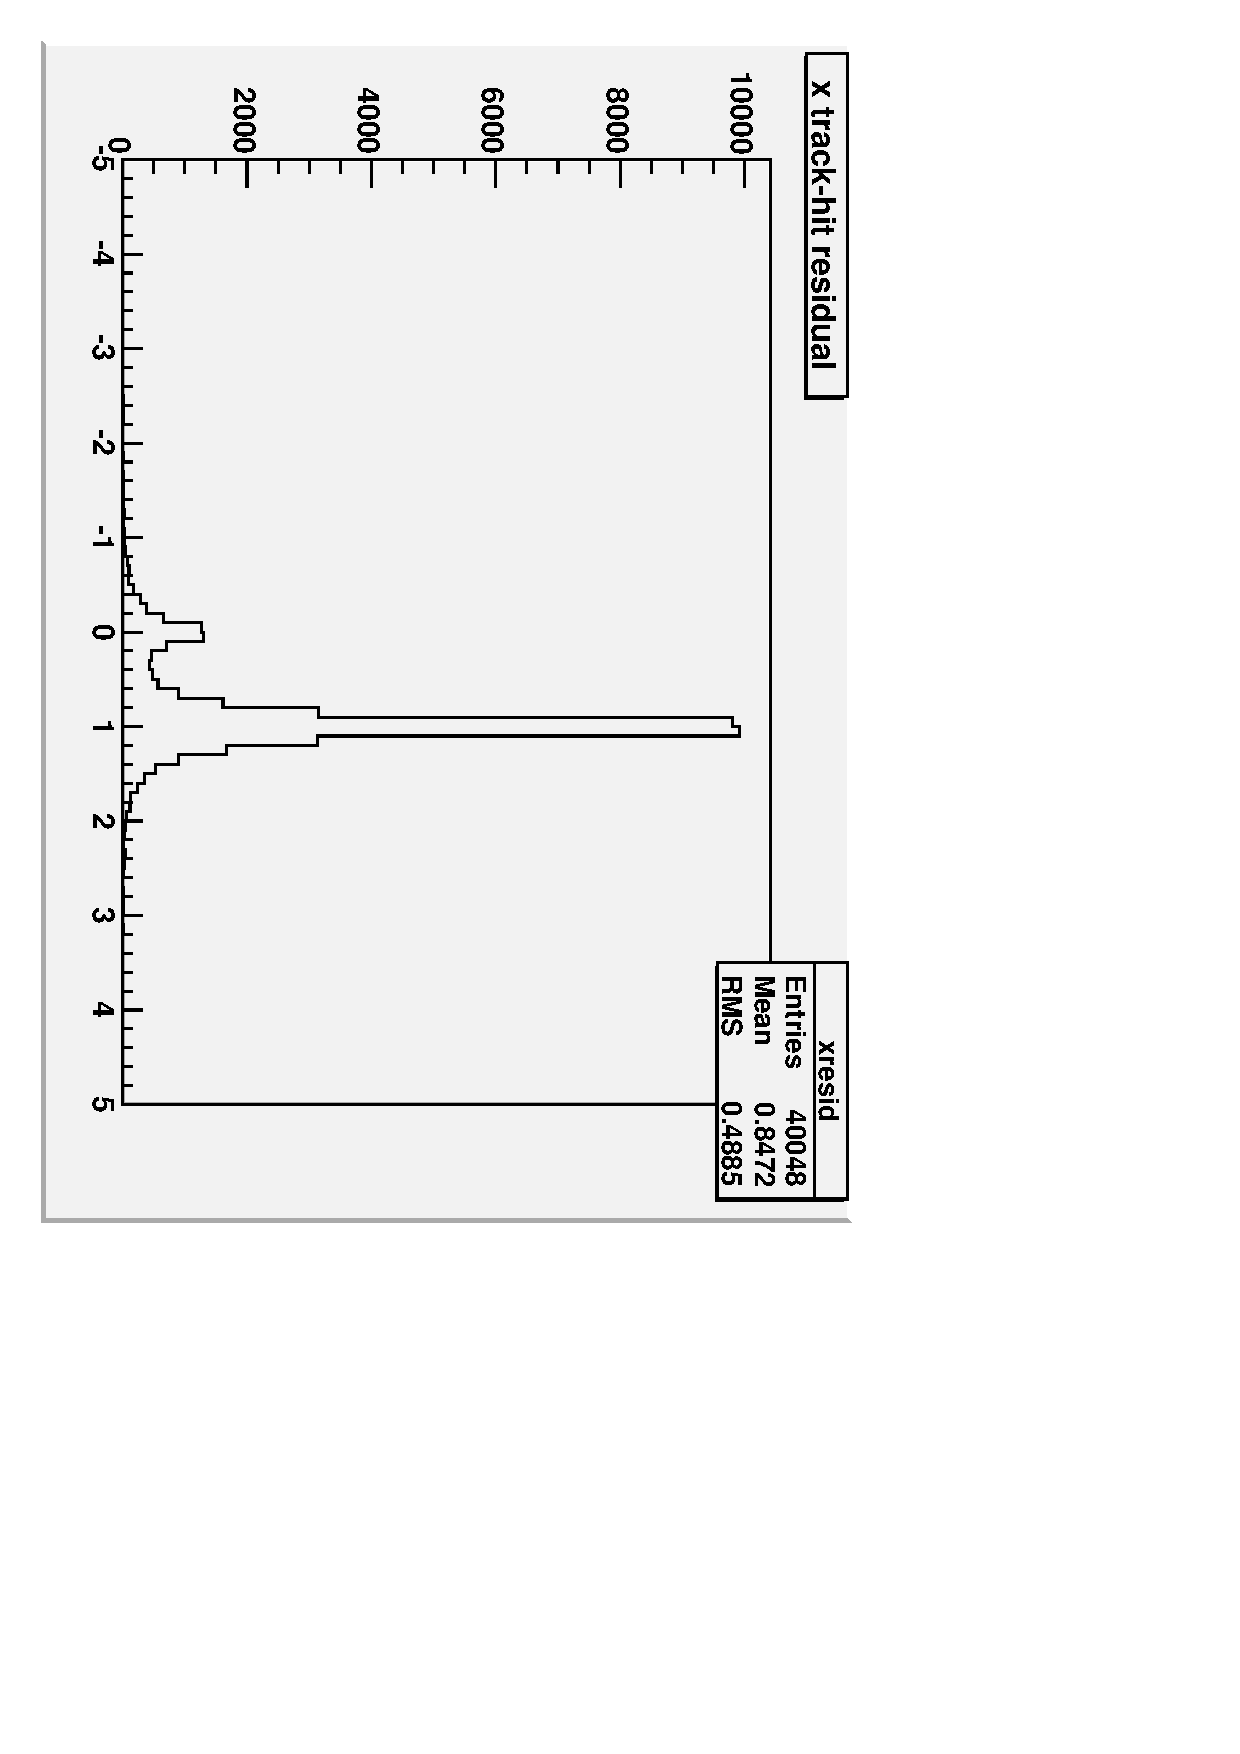
\includegraphics[height=\linewidth, angle=90]{xresid_deweighted_globalMuons.pdf}
  \end{minipage} \\
  \begin{minipage}{\linewidth}
  \end{minipage} & &
  \begin{minipage}{\linewidth}
    \begin{center}
      deweighted globalMuon
    \end{center}
  \end{minipage}
\end{tabular}
\end{center}
\end{frame}

\begin{frame}
\frametitle{Update!  10 pb$^{-1}$ deweighted globalMuon alignment}

\begin{center}
\begin{tabular}{p{0.4\linewidth} c p{0.4\linewidth}}
  \begin{minipage}{\linewidth}
    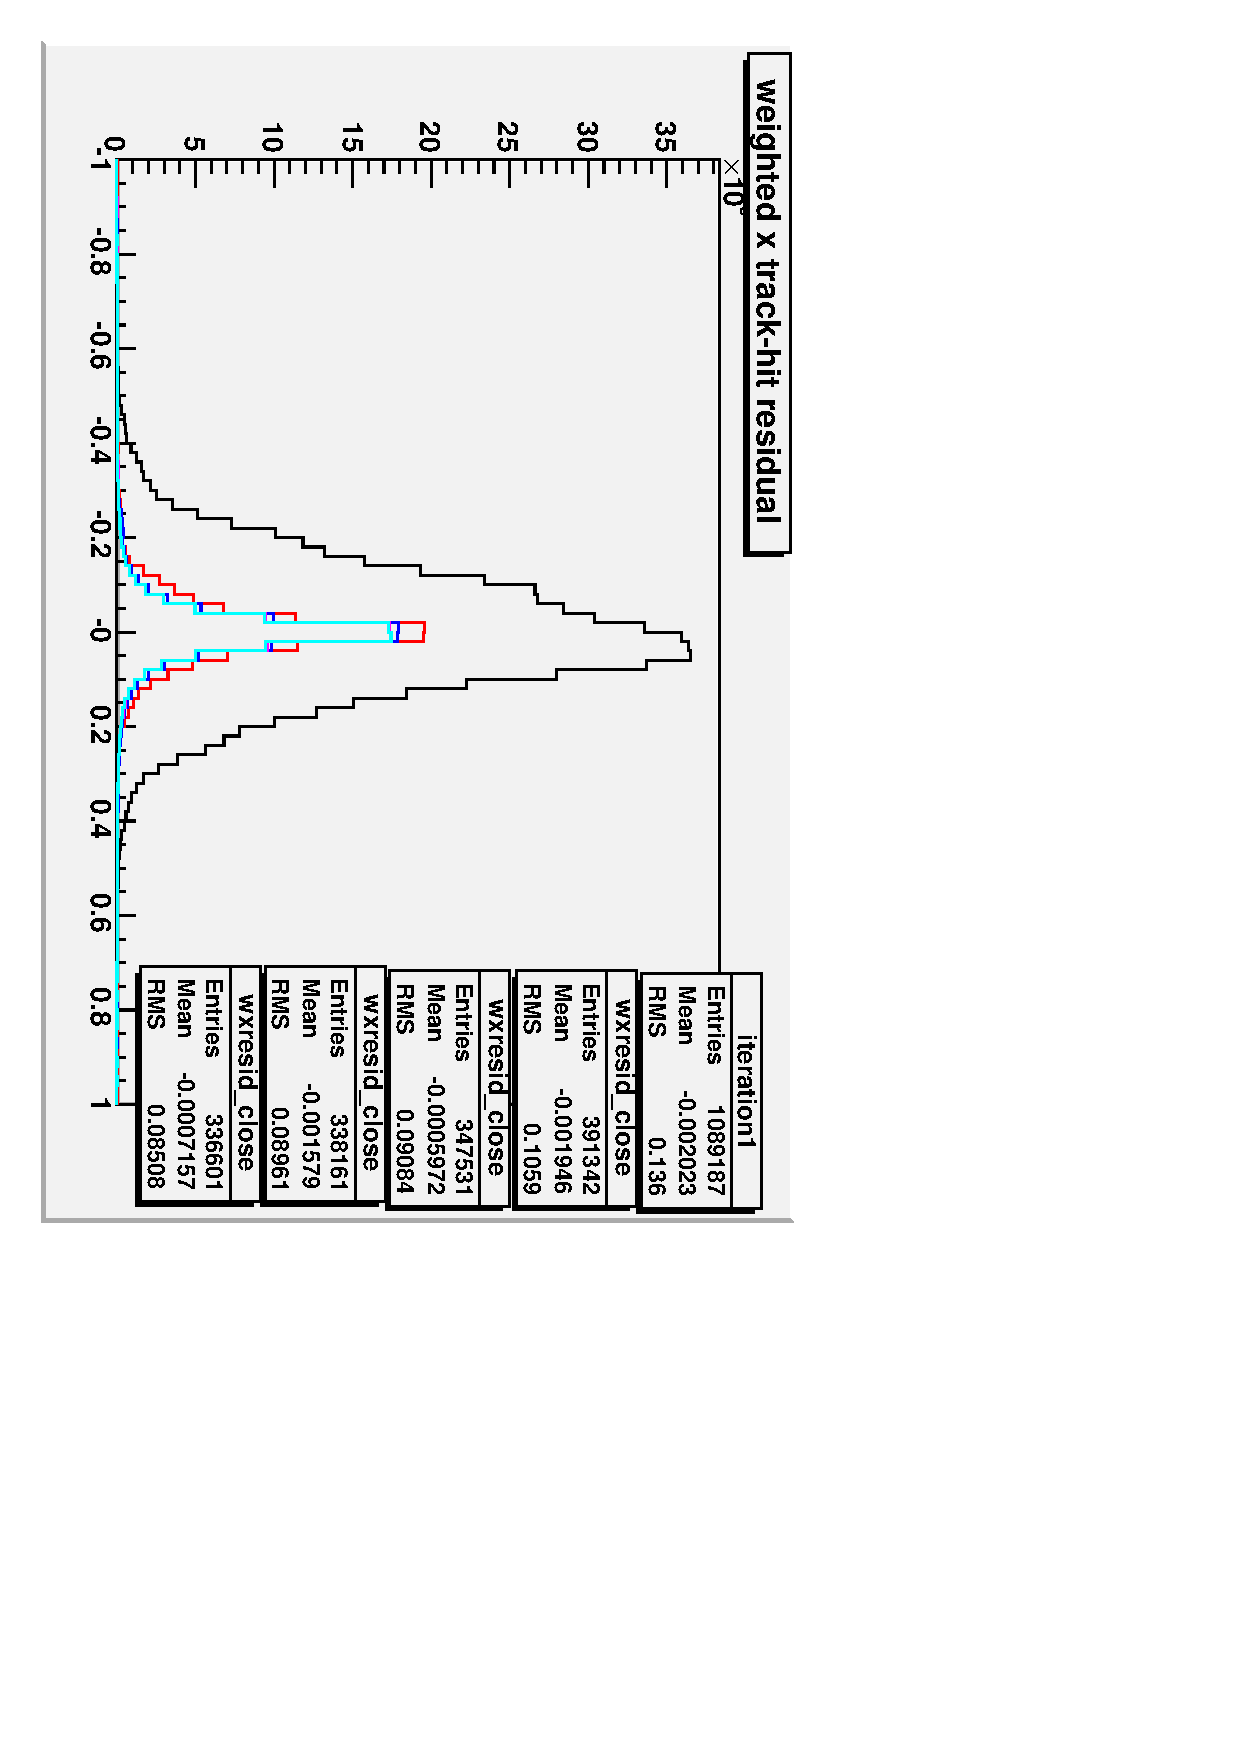
\includegraphics[height=\linewidth, angle=90]{wxresid_convergence.pdf}
  \end{minipage} & &
  \begin{minipage}{\linewidth}
    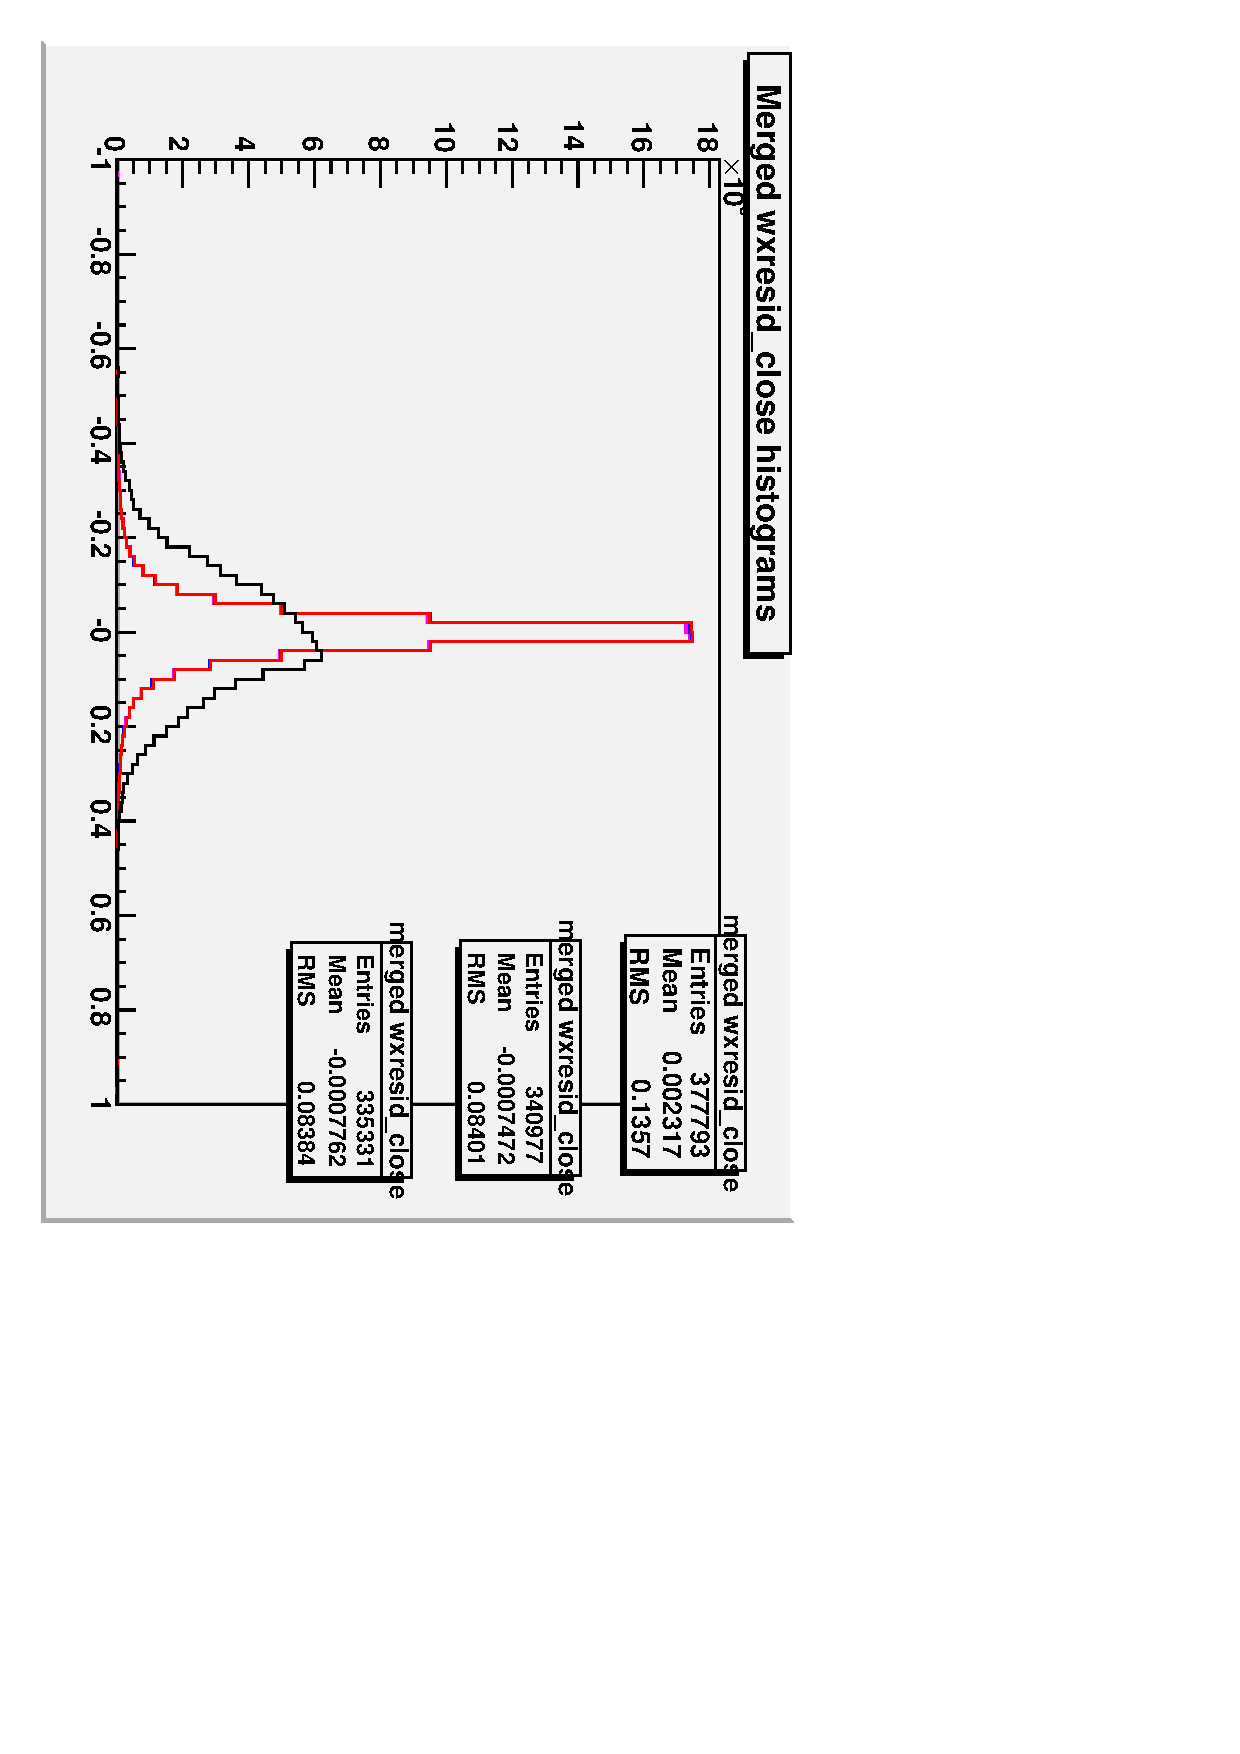
\includegraphics[height=\linewidth, angle=90]{wxresid_endcap_only.pdf}
  \end{minipage} \\
  \begin{minipage}{\linewidth}
    \begin{center}
      weighted x residual
    \end{center}
  \end{minipage} & &
  \begin{minipage}{\linewidth}
    \begin{center}
      endcap only (bug in DT)
    \end{center}
  \end{minipage} \\
  & & \\
  \begin{minipage}{\linewidth}
    \begin{center}
      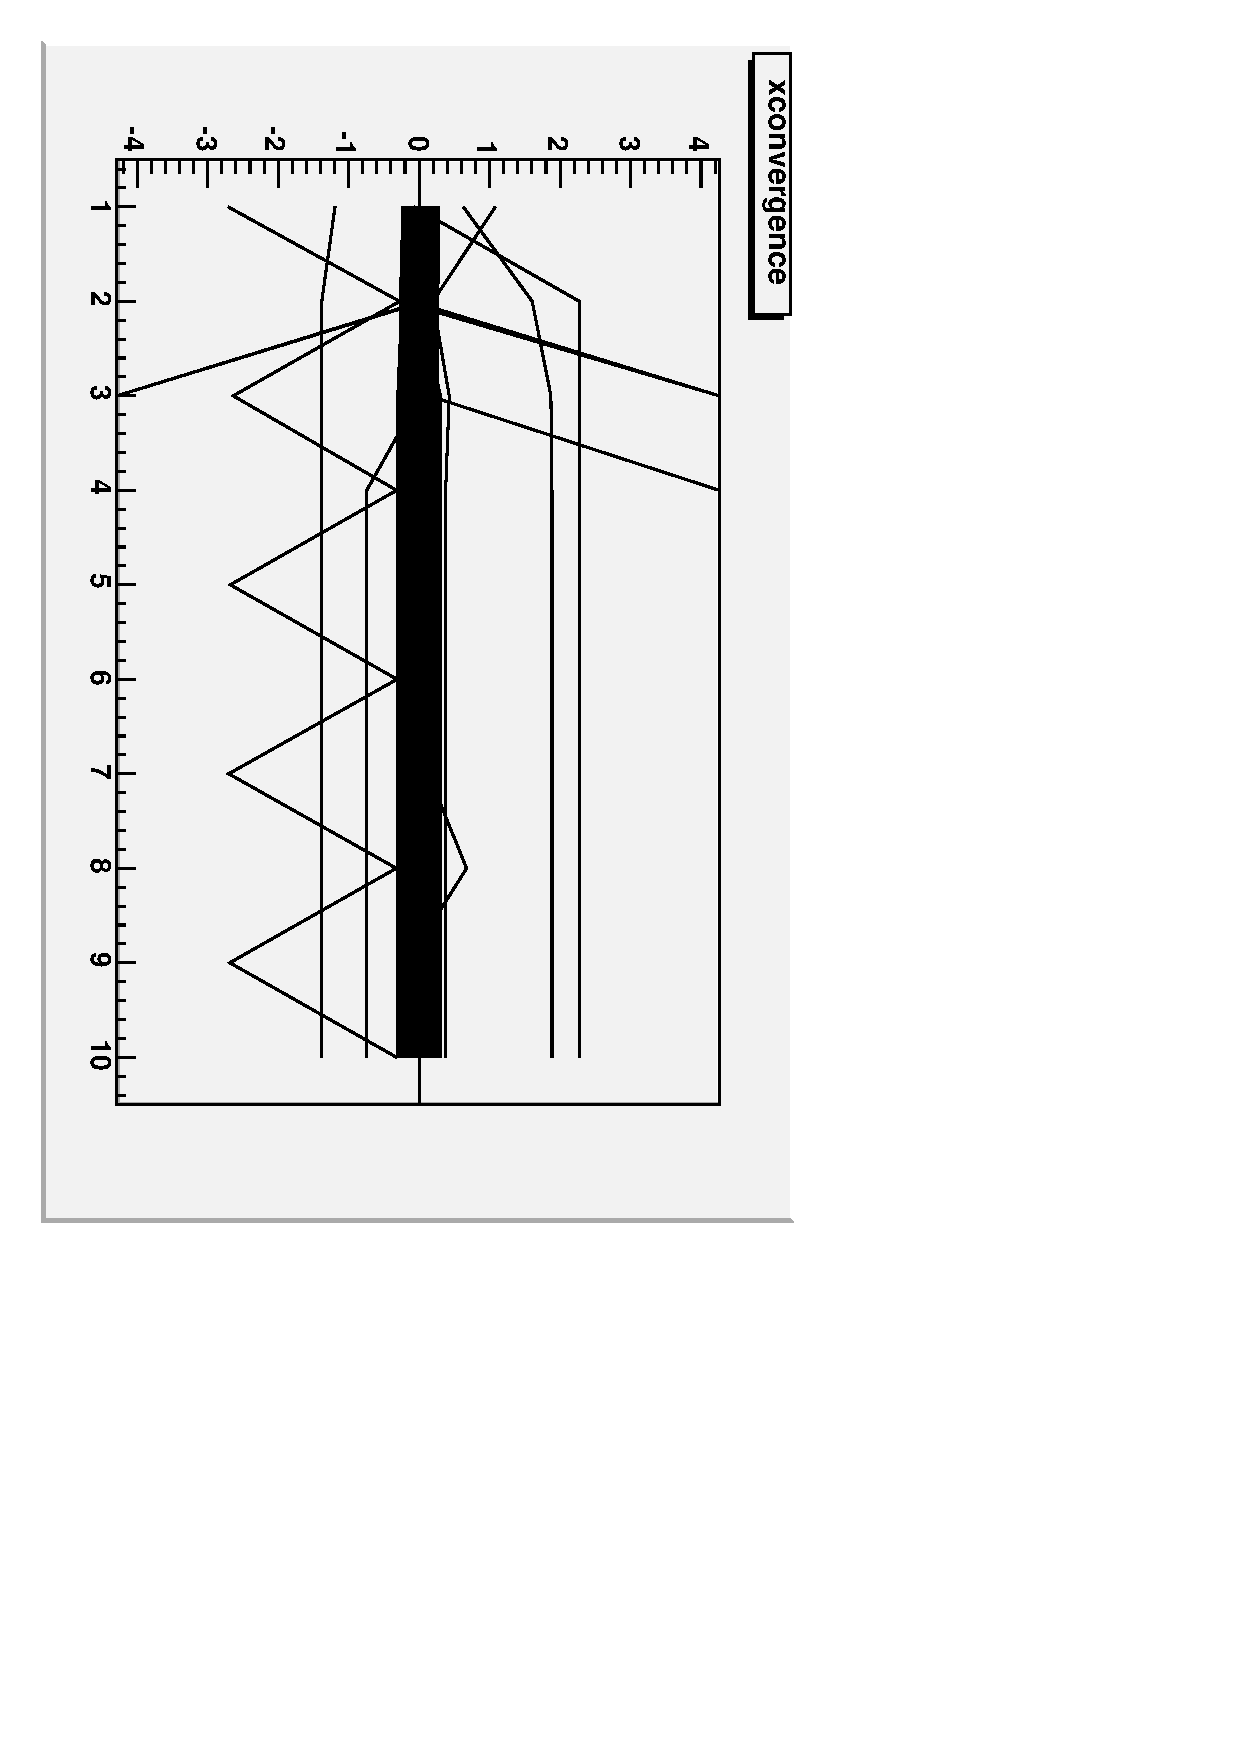
\includegraphics[height=\linewidth, angle=90]{xconvergence_still_looks_bad.pdf}
    \end{center}
  \end{minipage} & &
  \begin{minipage}{\linewidth}
      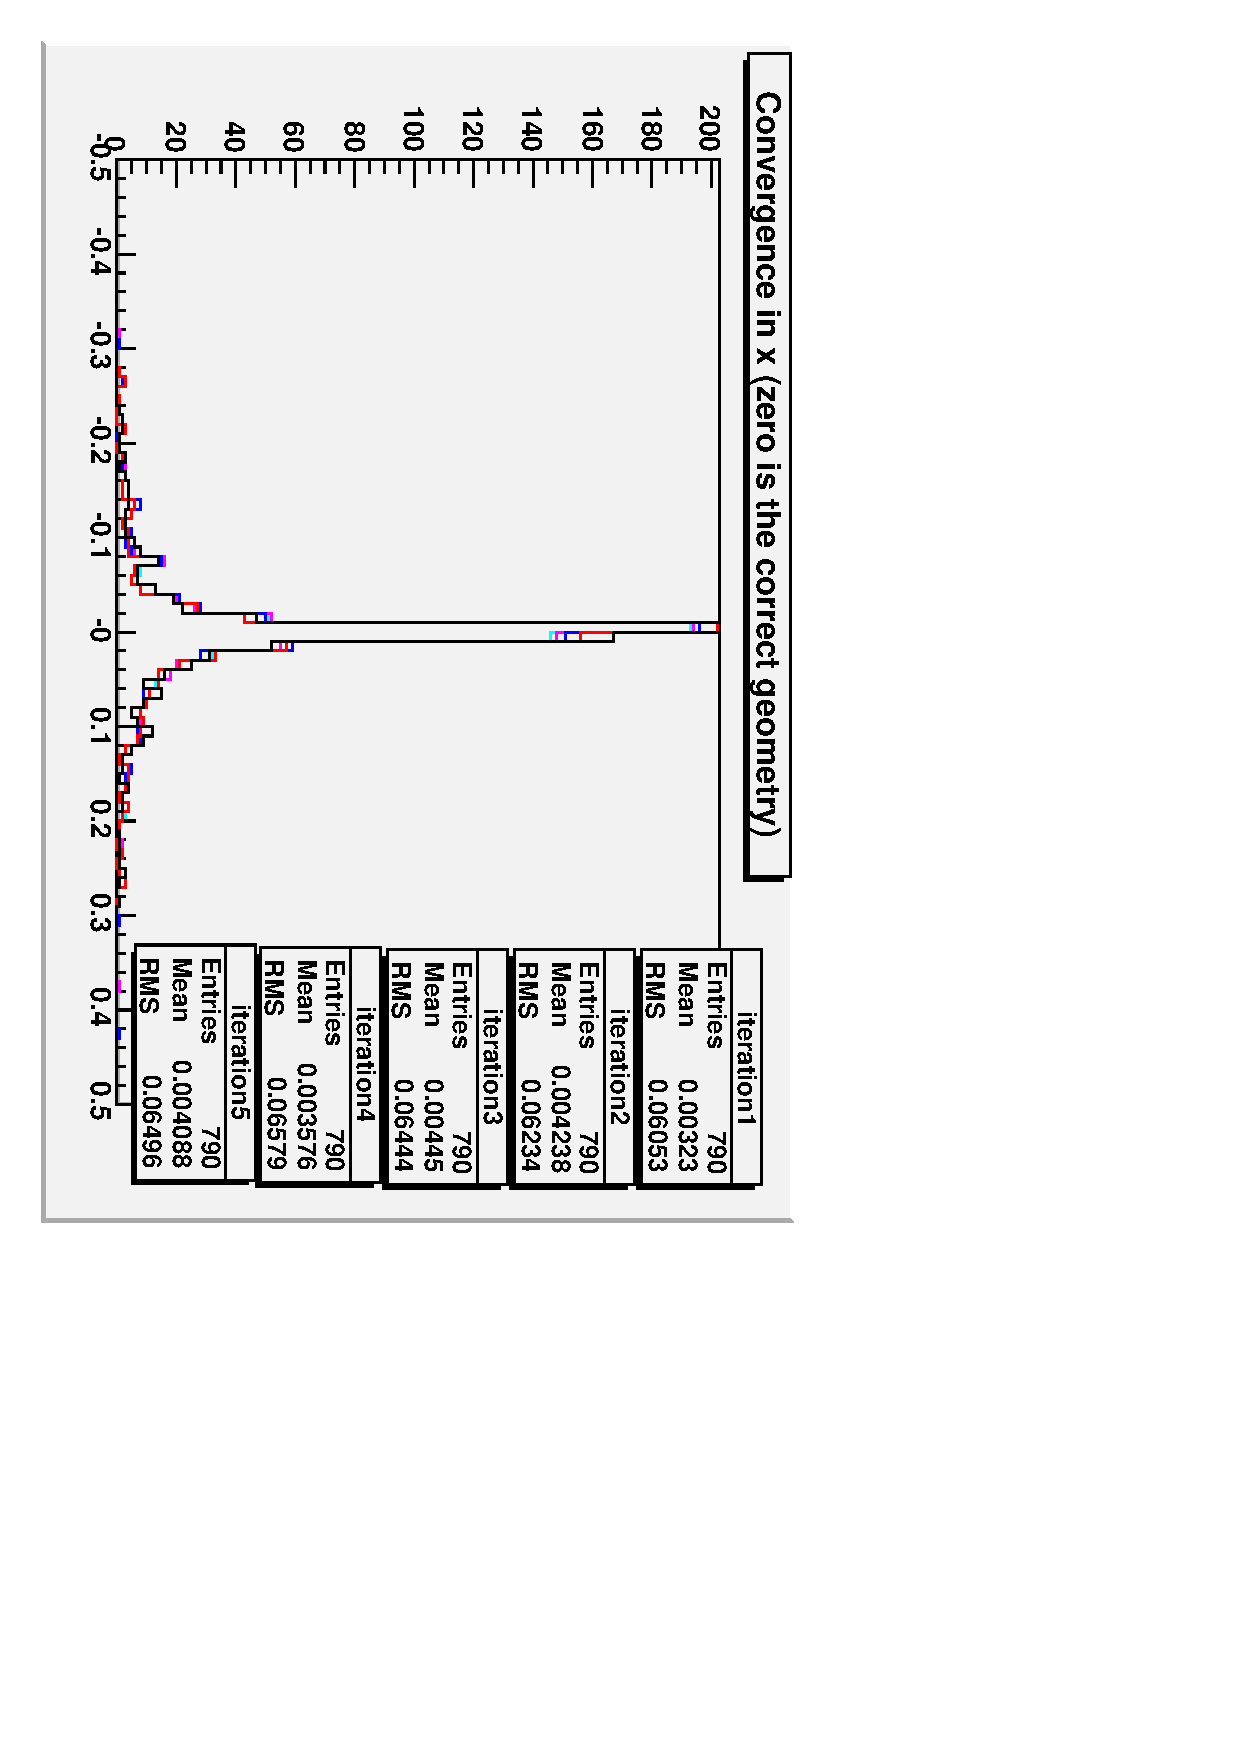
\includegraphics[height=\linewidth, angle=90]{xconvergence_still_looks_bad_hist.pdf}
  \end{minipage} \\
  \begin{minipage}{\linewidth}
    \begin{center}
      convergence still bad?
    \end{center}
  \end{minipage} & &
  \begin{minipage}{\linewidth}
    \begin{center}

    \end{center}
  \end{minipage}
\end{tabular}
\end{center}
\end{frame}

\begin{frame}
\frametitle{Updated update!  10 pb$^{-1}$ deweighted globalMuon}

\begin{center}
\begin{tabular}{p{0.4\linewidth} c p{0.4\linewidth}}
  \begin{minipage}{\linewidth}
    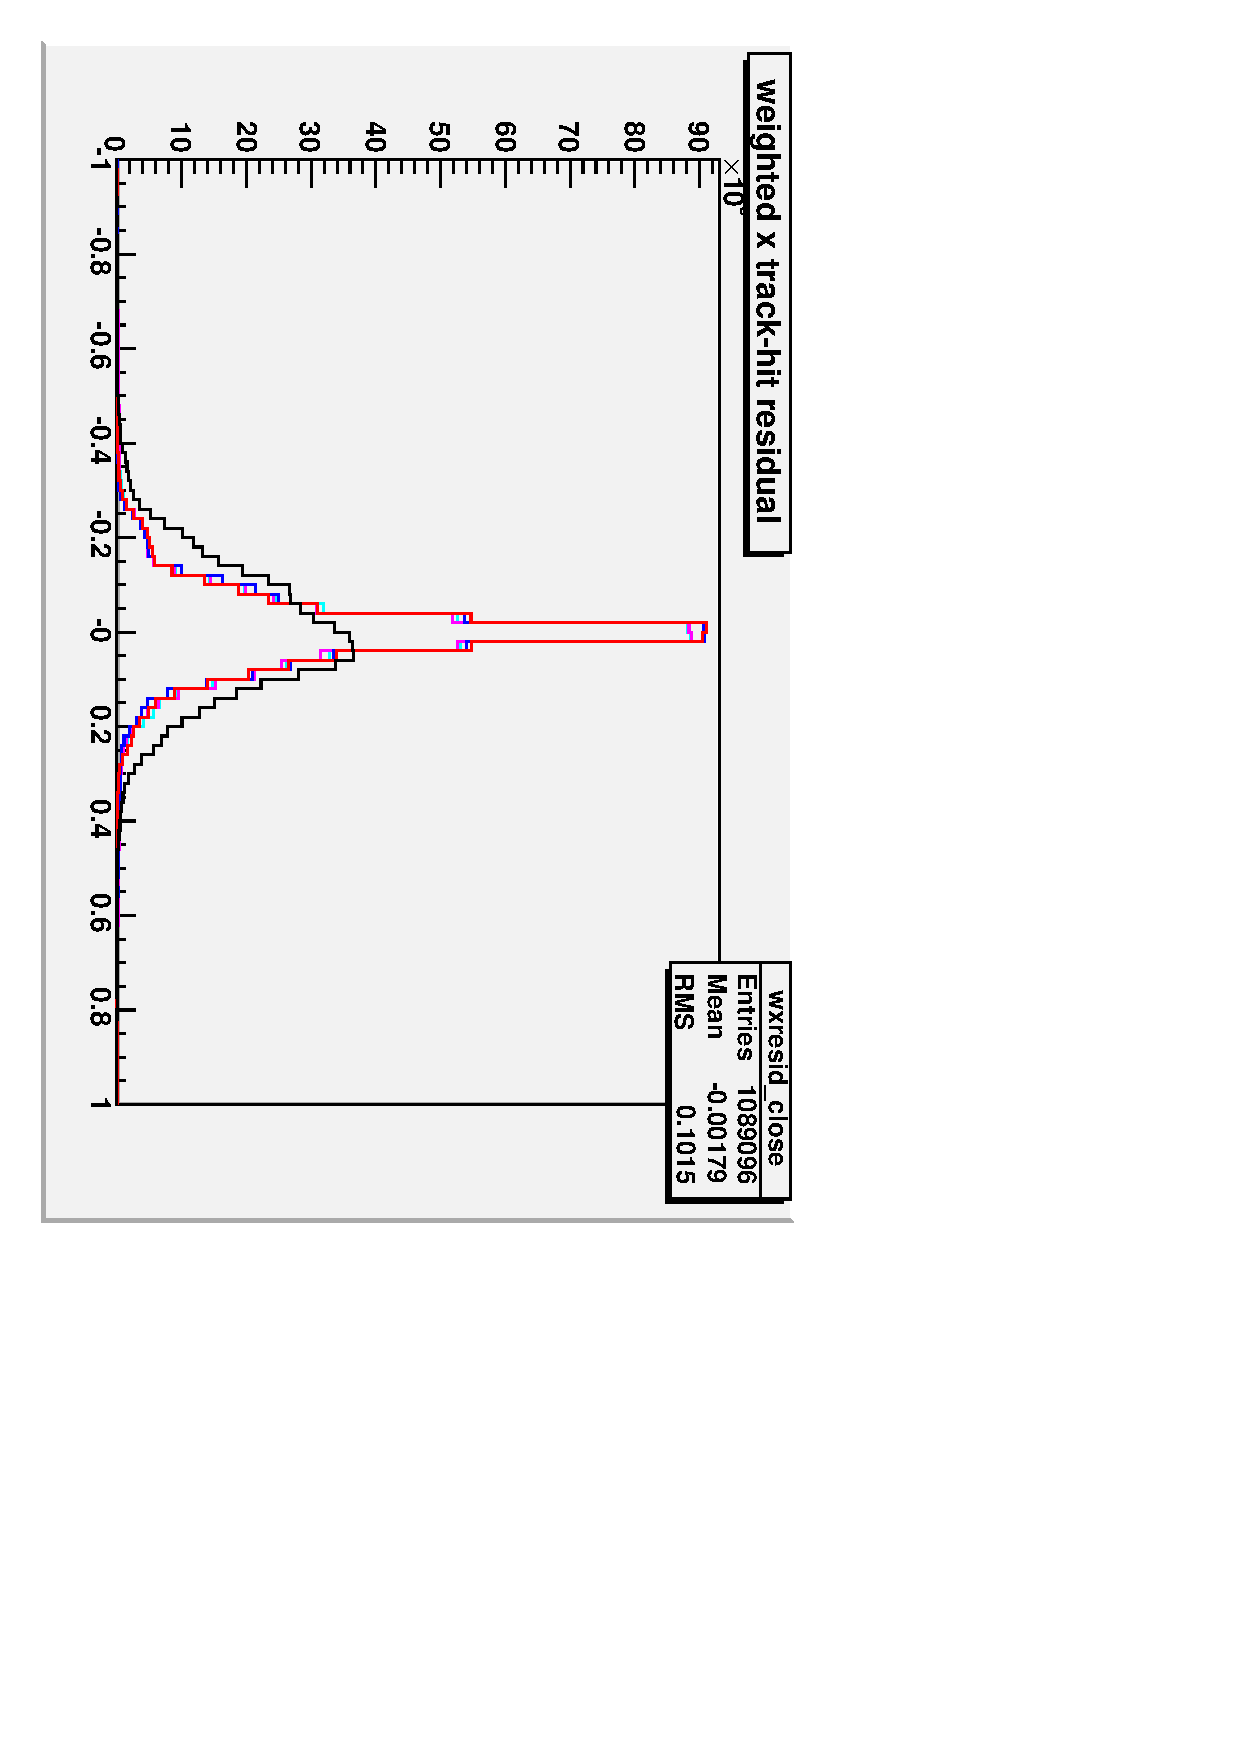
\includegraphics[height=\linewidth, angle=90]{wxresid_convergence_workingDT.pdf}
  \end{minipage} & &
  \begin{minipage}{\linewidth}
  \end{minipage} \\
  \begin{minipage}{\linewidth}
    \begin{center}
      weighted x residual
    \end{center}
  \end{minipage} & &
  \begin{minipage}{\linewidth}
    \begin{center}
      (no bug in DT)
    \end{center}
  \end{minipage} \\
  & & \\
  \begin{minipage}{\linewidth}
    \begin{center}
      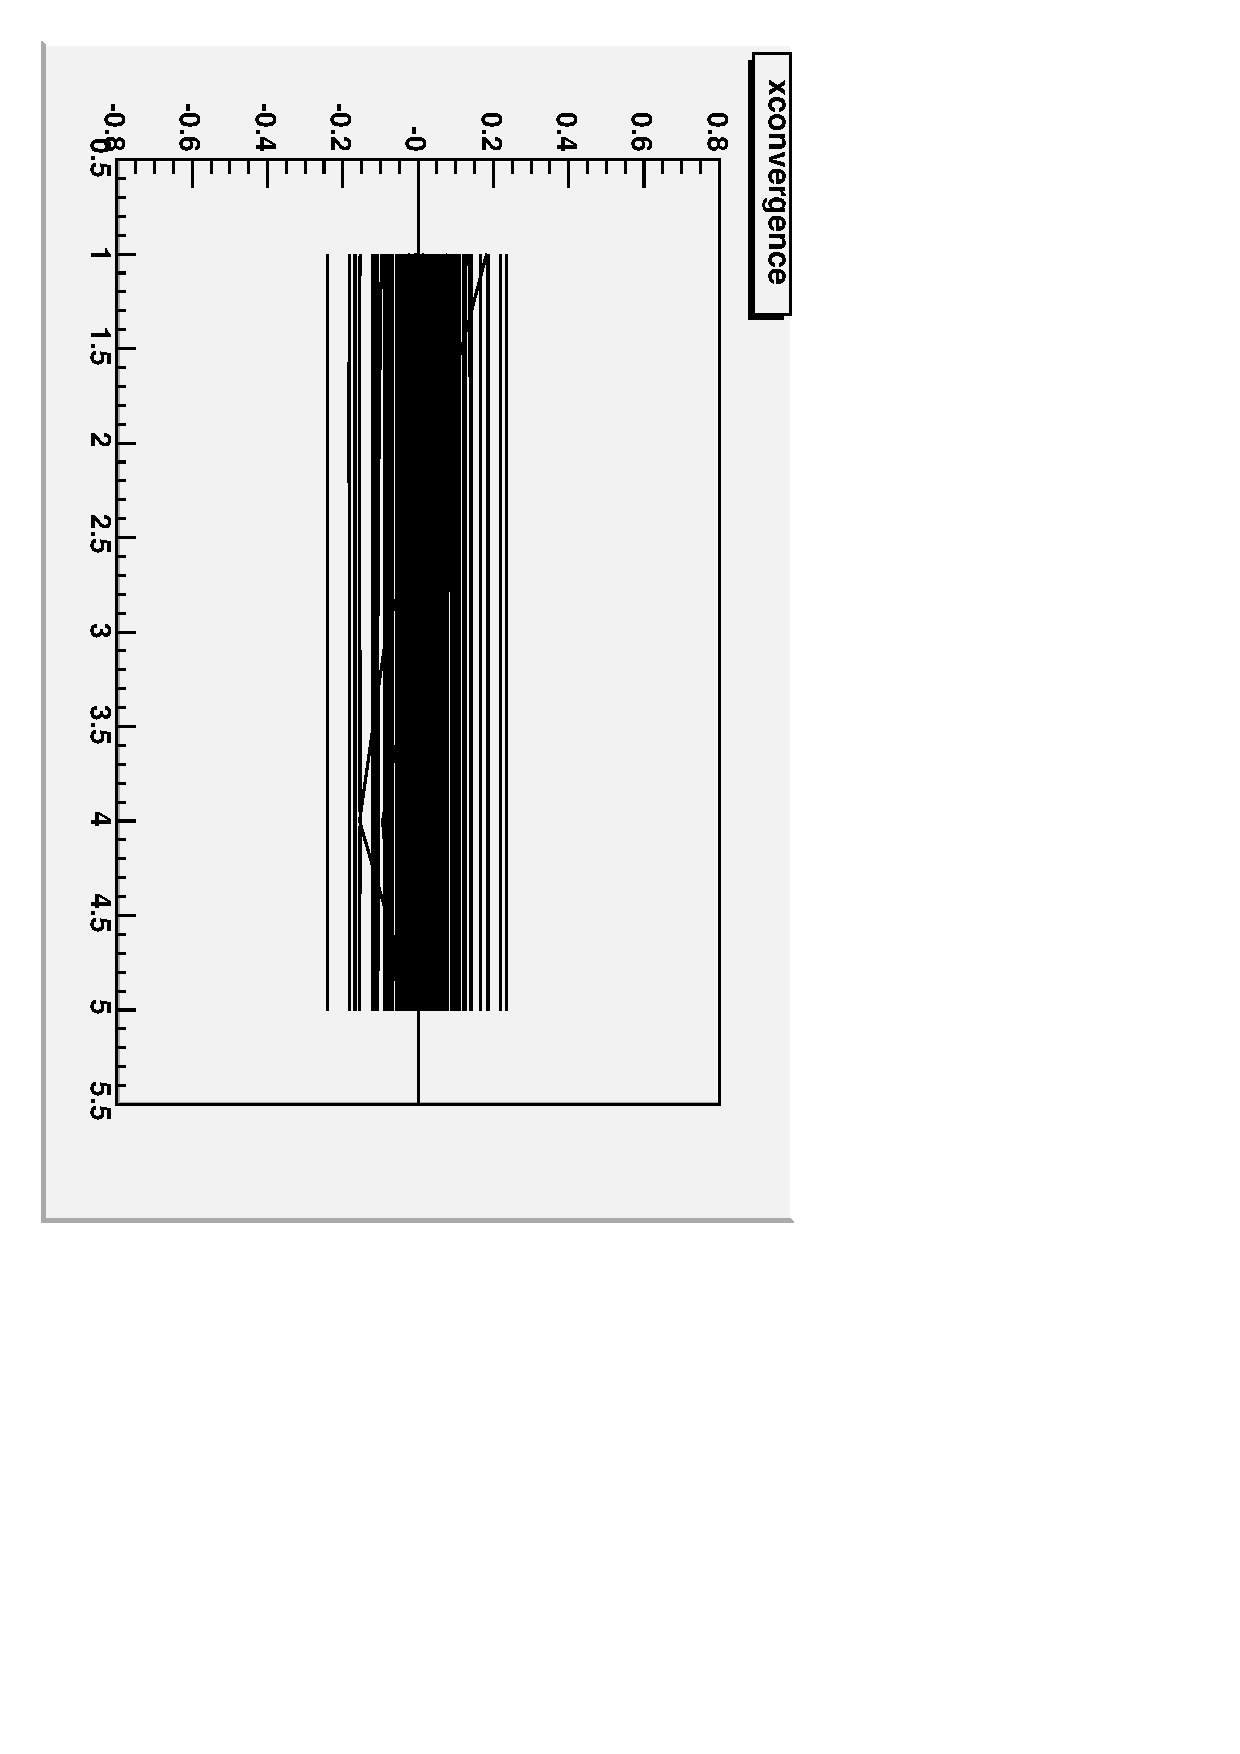
\includegraphics[height=\linewidth, angle=90]{convergence_is_all_in_iter1_lines.pdf}
    \end{center}
  \end{minipage} & &
  \begin{minipage}{\linewidth}
      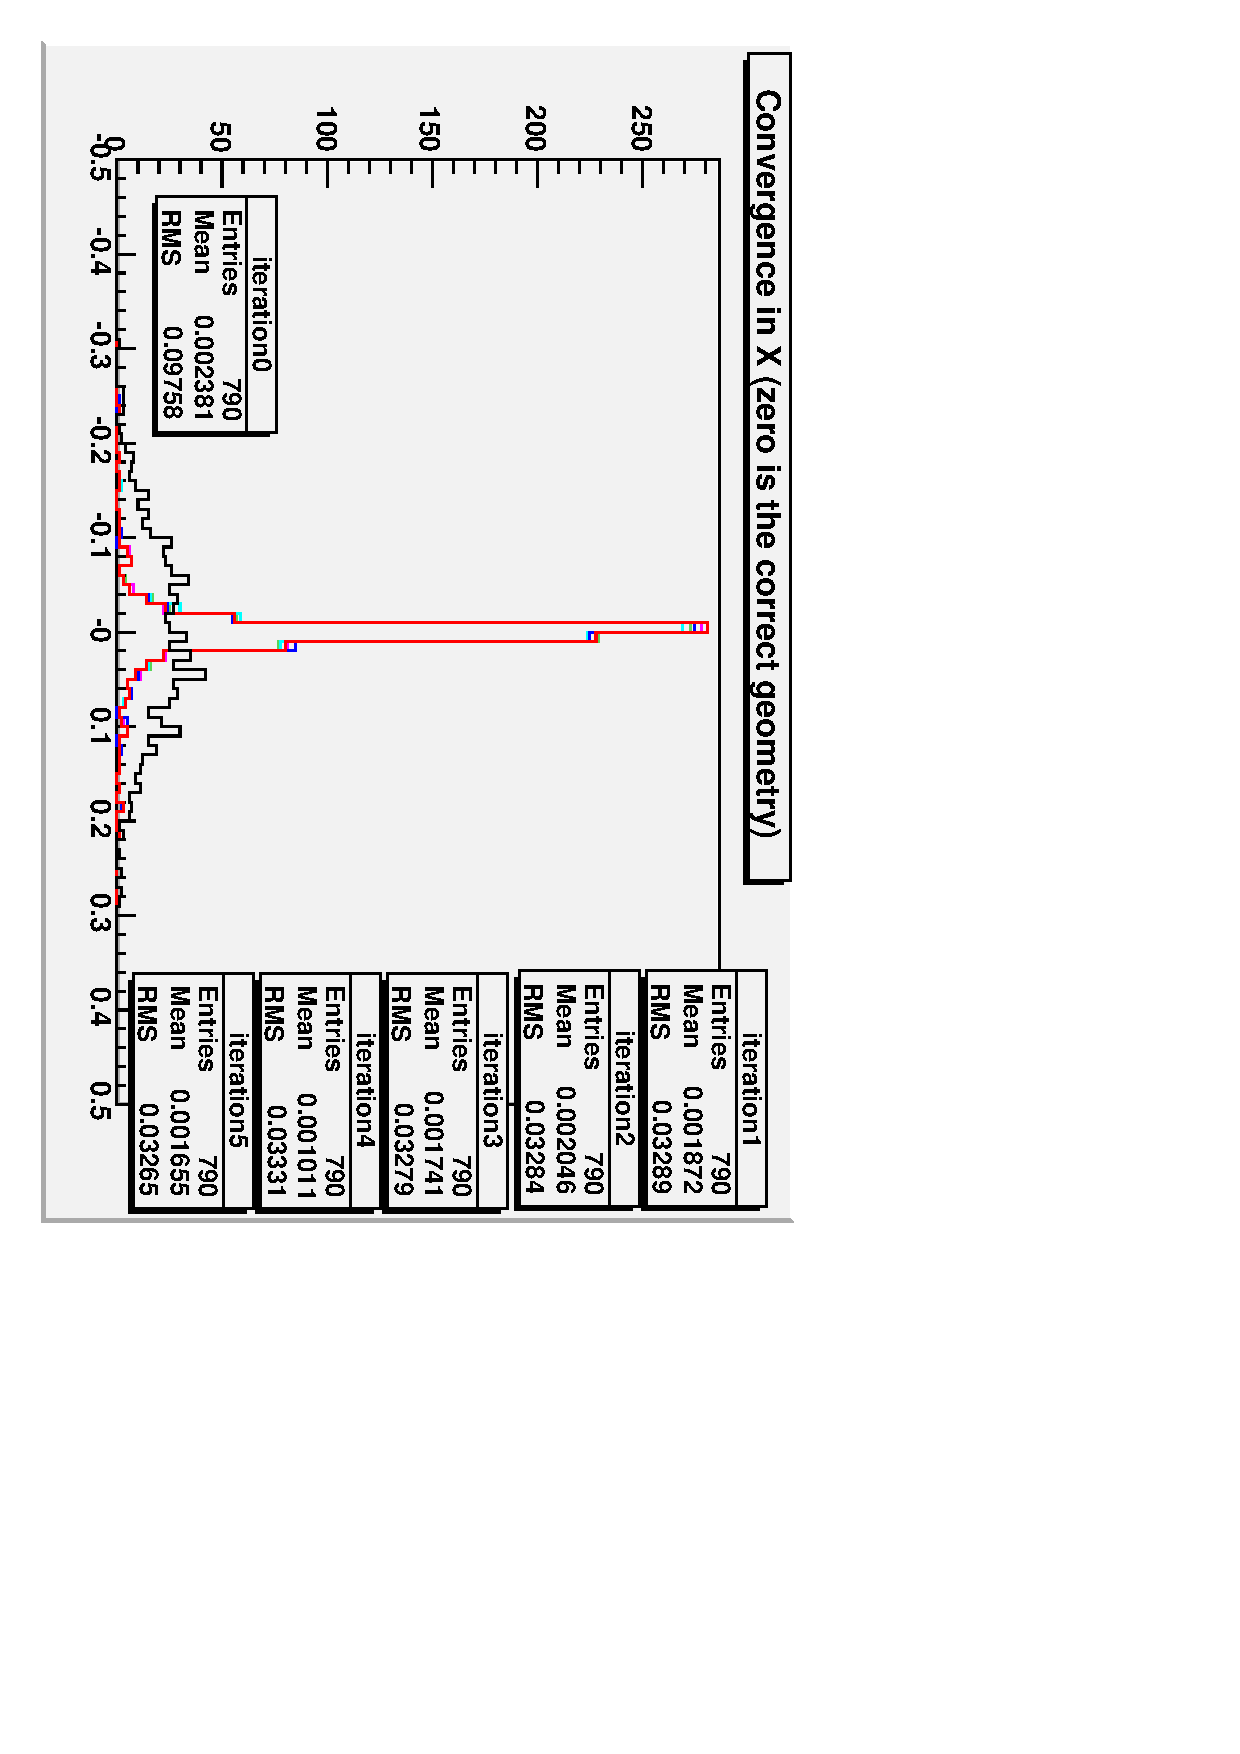
\includegraphics[height=\linewidth, angle=90]{convergence_is_all_in_iter1.pdf}
  \end{minipage} \\
  \begin{minipage}{\linewidth}
    \begin{center}
      flat convergence
    \end{center}
  \end{minipage} & &
  \begin{minipage}{\linewidth}
    \begin{center}
      it's all in iteration 1
    \end{center}
  \end{minipage}
\end{tabular}
\end{center}
\end{frame}

\begin{frame}
\frametitle{Raw output from this {\it super-preliminary} alignment}

Alignment accuracy (RMS of aligned minus true)
\begin{center}
\begin{tabular}{c | c p{2 cm} c | c}
& DT & & & CSC \\
$x$ & 500 $\mu$m & & $x$ & 200 $\mu$m \\
$y$ & 700 $\mu$m & & $y$ & 4 mm \\
$z$ & 1 mm & & $z$ & 1.6 cm \\
$\phi_x$ & 16 mrad & & $\phi_x$ & 10 mrad \\
$\phi_y$ & 3 mrad & & $\phi_y$ & 2 mrad \\
$\phi_z$ & 0.5 mrad & & $\phi_z$ & 1 mrad \\
\end{tabular}
\end{center}

\vfill
Alignment precision: self-evident bugs

\vfill
$x$ residuals, post alignment: 1 mm RMS in barrel, 750 microns endcap
\end{frame}

\begin{frame}
\frametitle{MTCC alignments}

Exercise AlignmentProducer monitoring (the ``sanity checks'' tool) \mbox{\hspace{-1 cm}}
\begin{itemize}
\item e.g.\ select alignment monitoring histograms with $>$ 0 entries:
\end{itemize}

\begin{center}
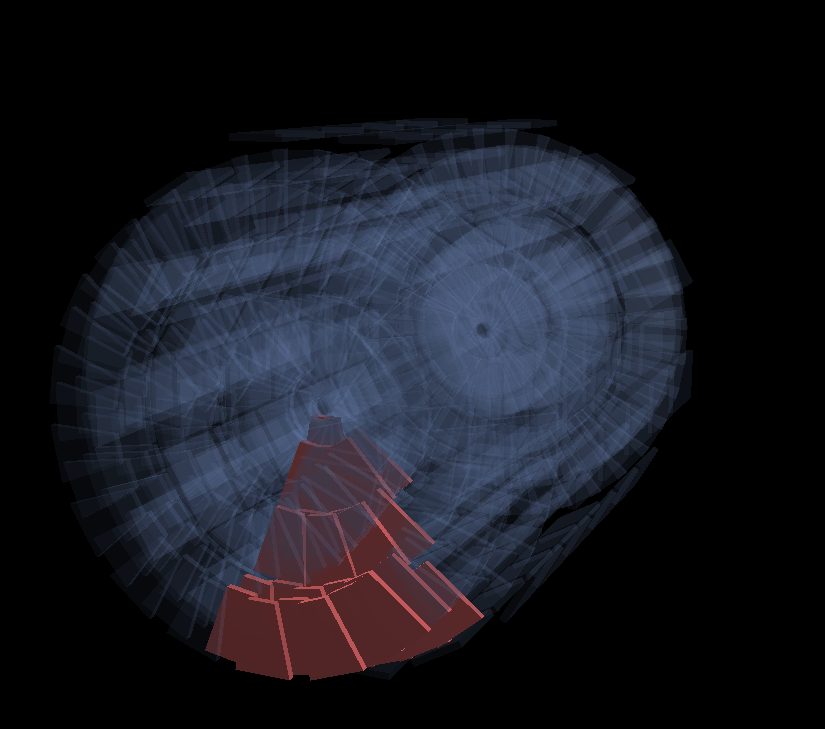
\includegraphics[width=0.5\linewidth]{mtcc_chambers.png}
\end{center}

\vspace{-0.25 cm}
\begin{itemize}
\item searched for peculiar features\ldots (skipping detective story)
\end{itemize}
\end{frame}

\begin{frame}
\frametitle{Selected histograms with $\int_3^5 |\mbox{yresid}| / \int_0^5 |\mbox{yresid}| > $ 0.2}
\begin{center}
\begin{tabular}{p{0.5\linewidth} p{0.5\linewidth}}
\begin{minipage}{\linewidth}
Result: all ME+1/3 and only \\
\mbox{ } \hfill ME+1/3

\vspace{0.5 cm}
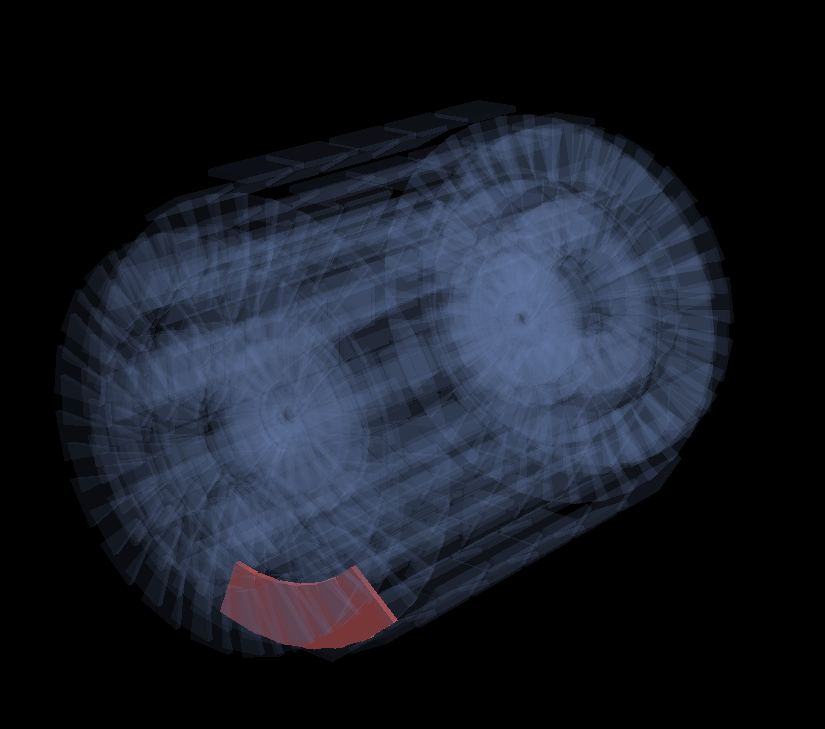
\includegraphics[width=\linewidth]{affected_chambers.png}
\end{minipage} &
\begin{minipage}{\linewidth}
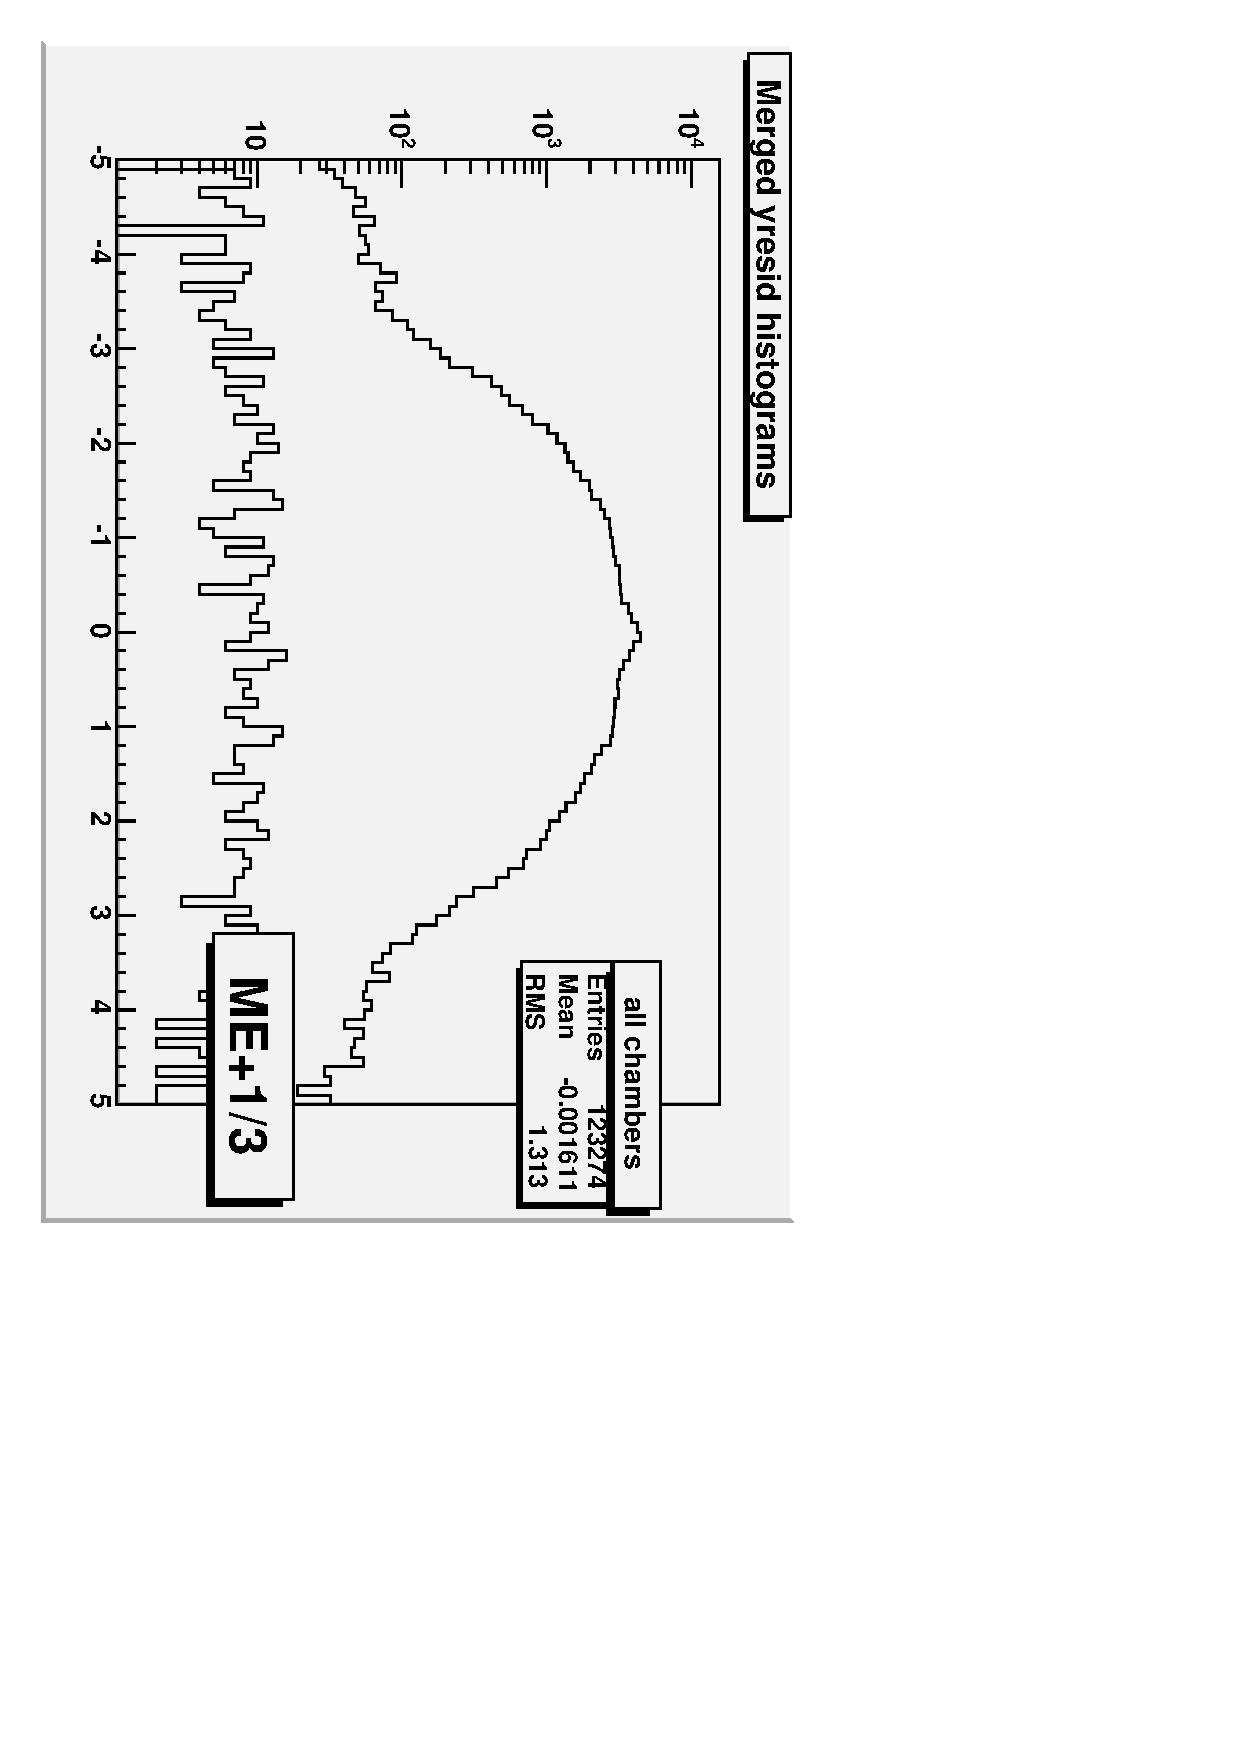
\includegraphics[height=\linewidth, angle=90]{affected_chambers_yresid.pdf} \\
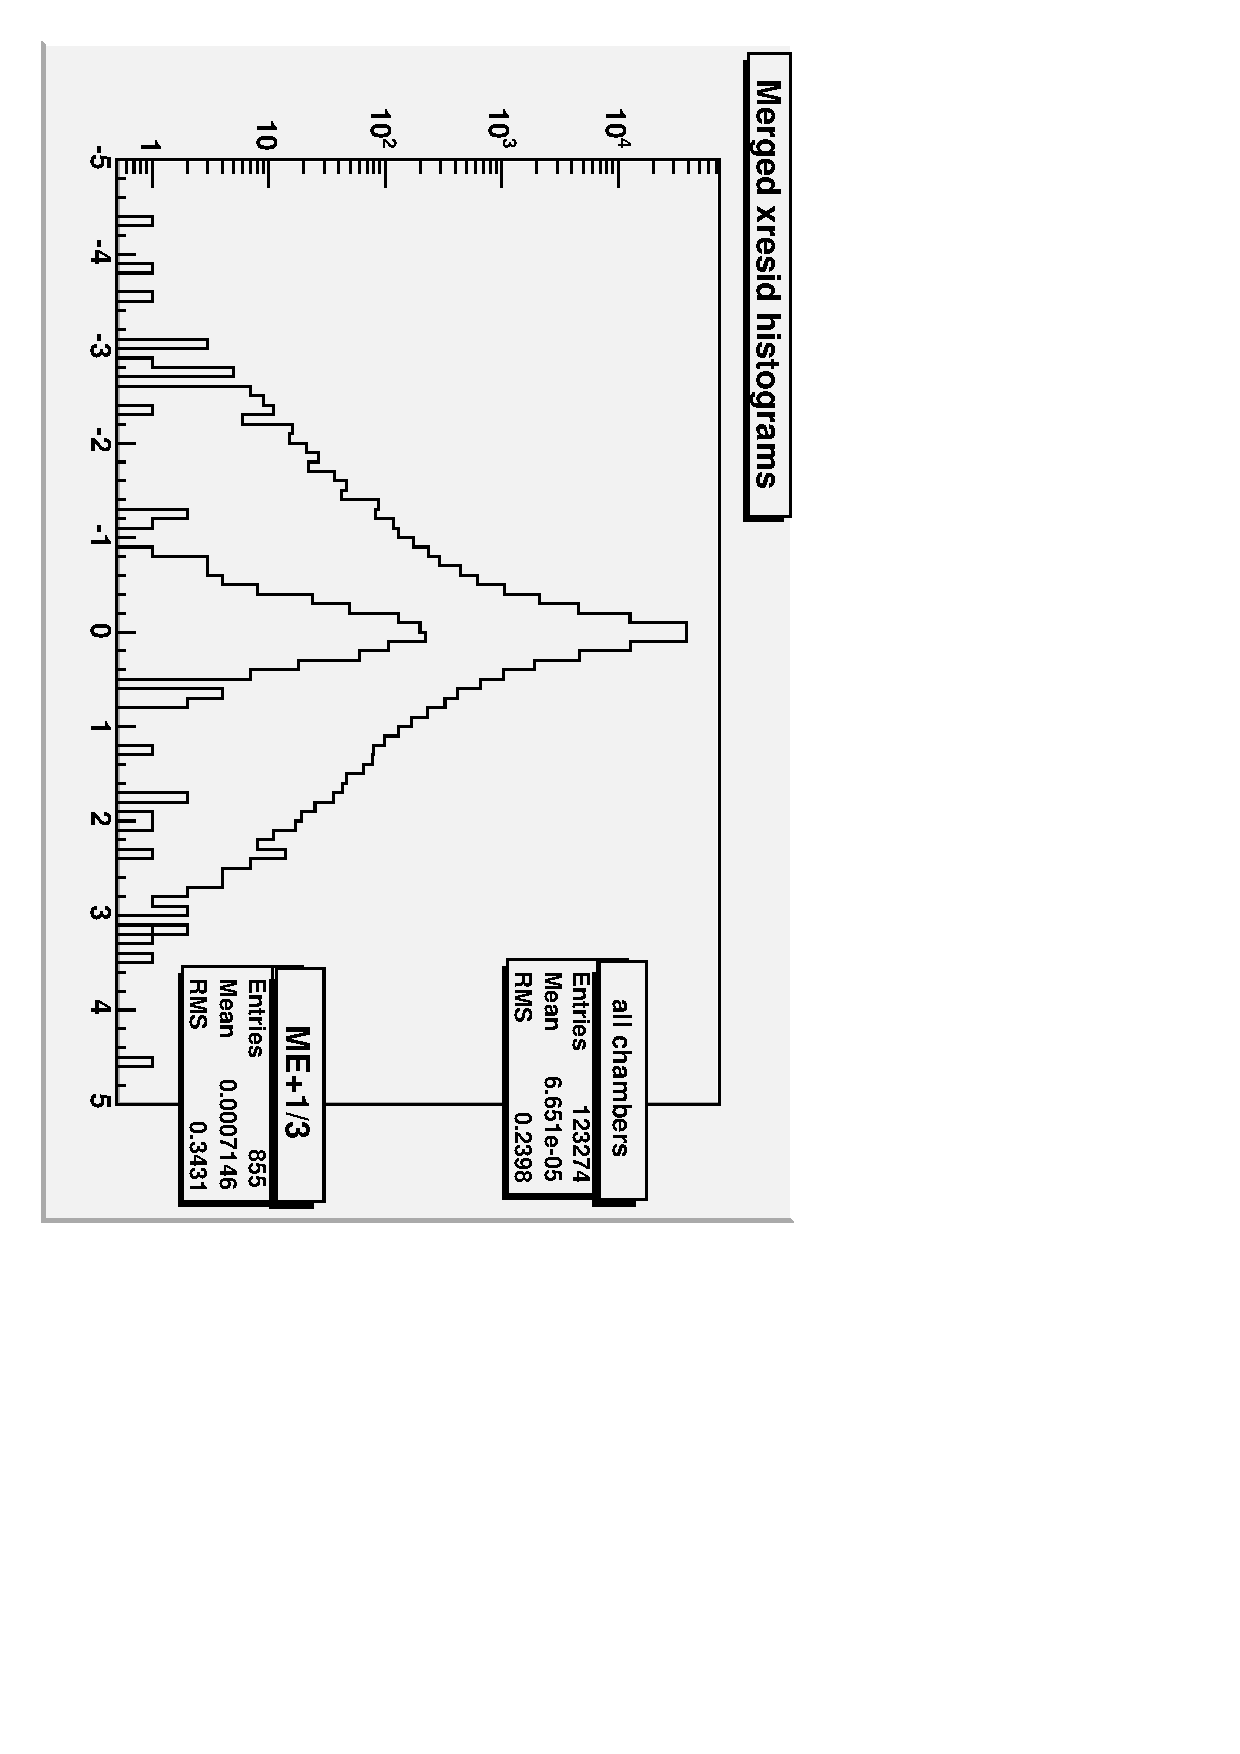
\includegraphics[height=\linewidth, angle=90]{affected_chambers_xresid.pdf}
\end{minipage}
\end{tabular}
\end{center}
\end{frame}

\begin{frame}
\frametitle{Looks like noisy wires?}
\begin{center}
\begin{tabular}{p{0.4\linewidth} p{0.5\linewidth}}
\begin{minipage}{\linewidth}
\begin{center}
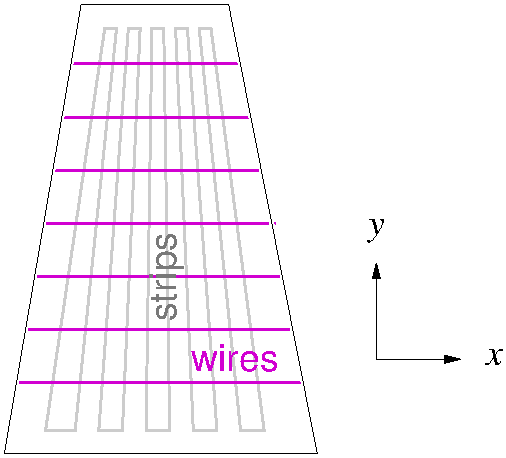
\includegraphics[width=0.85\linewidth]{orientations.pdf}

\begin{itemize}
  \item Only one run tested: 00003797
  \item $\vec{B}$ = 0
  \item $x$ residuals look normal
\end{itemize}
\end{center}
\end{minipage} &
\begin{minipage}{\linewidth}
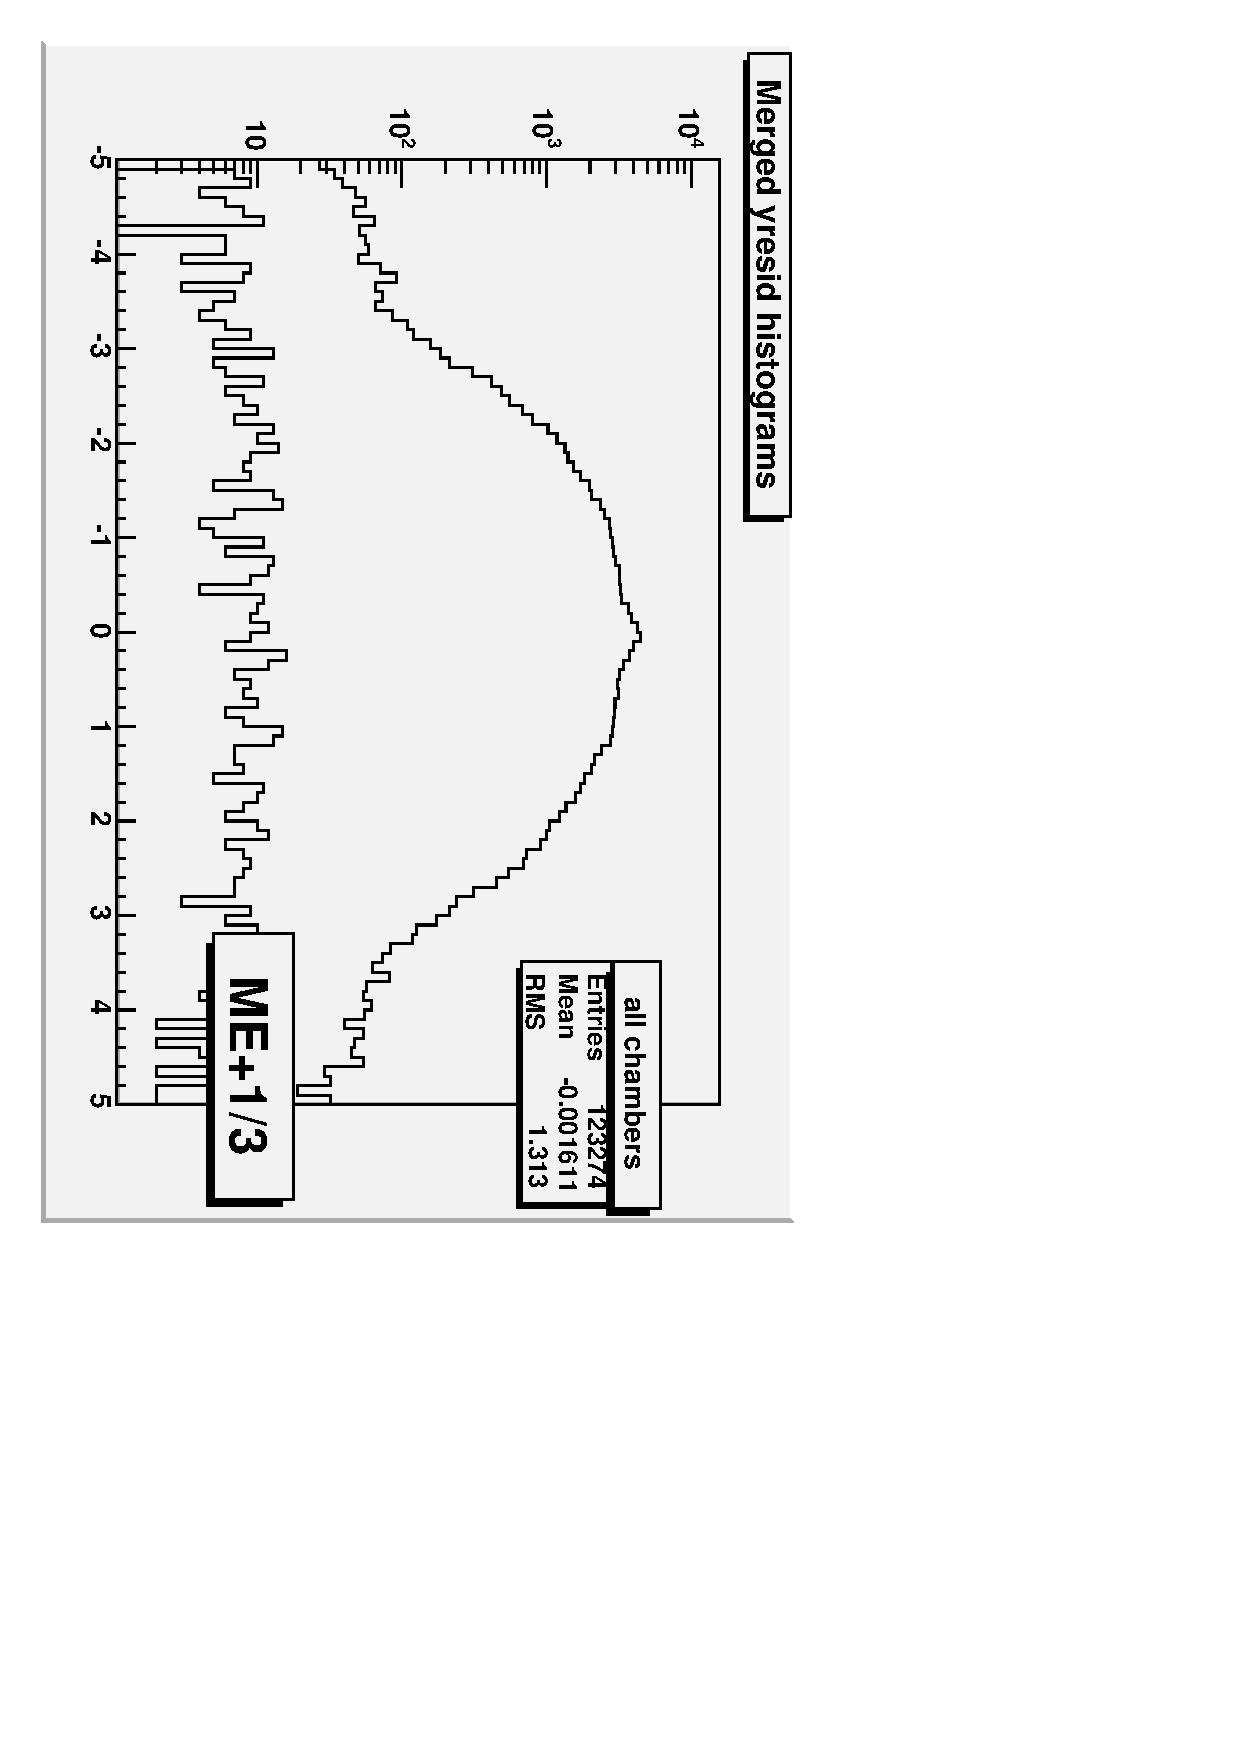
\includegraphics[height=\linewidth, angle=90]{affected_chambers_yresid.pdf} \\
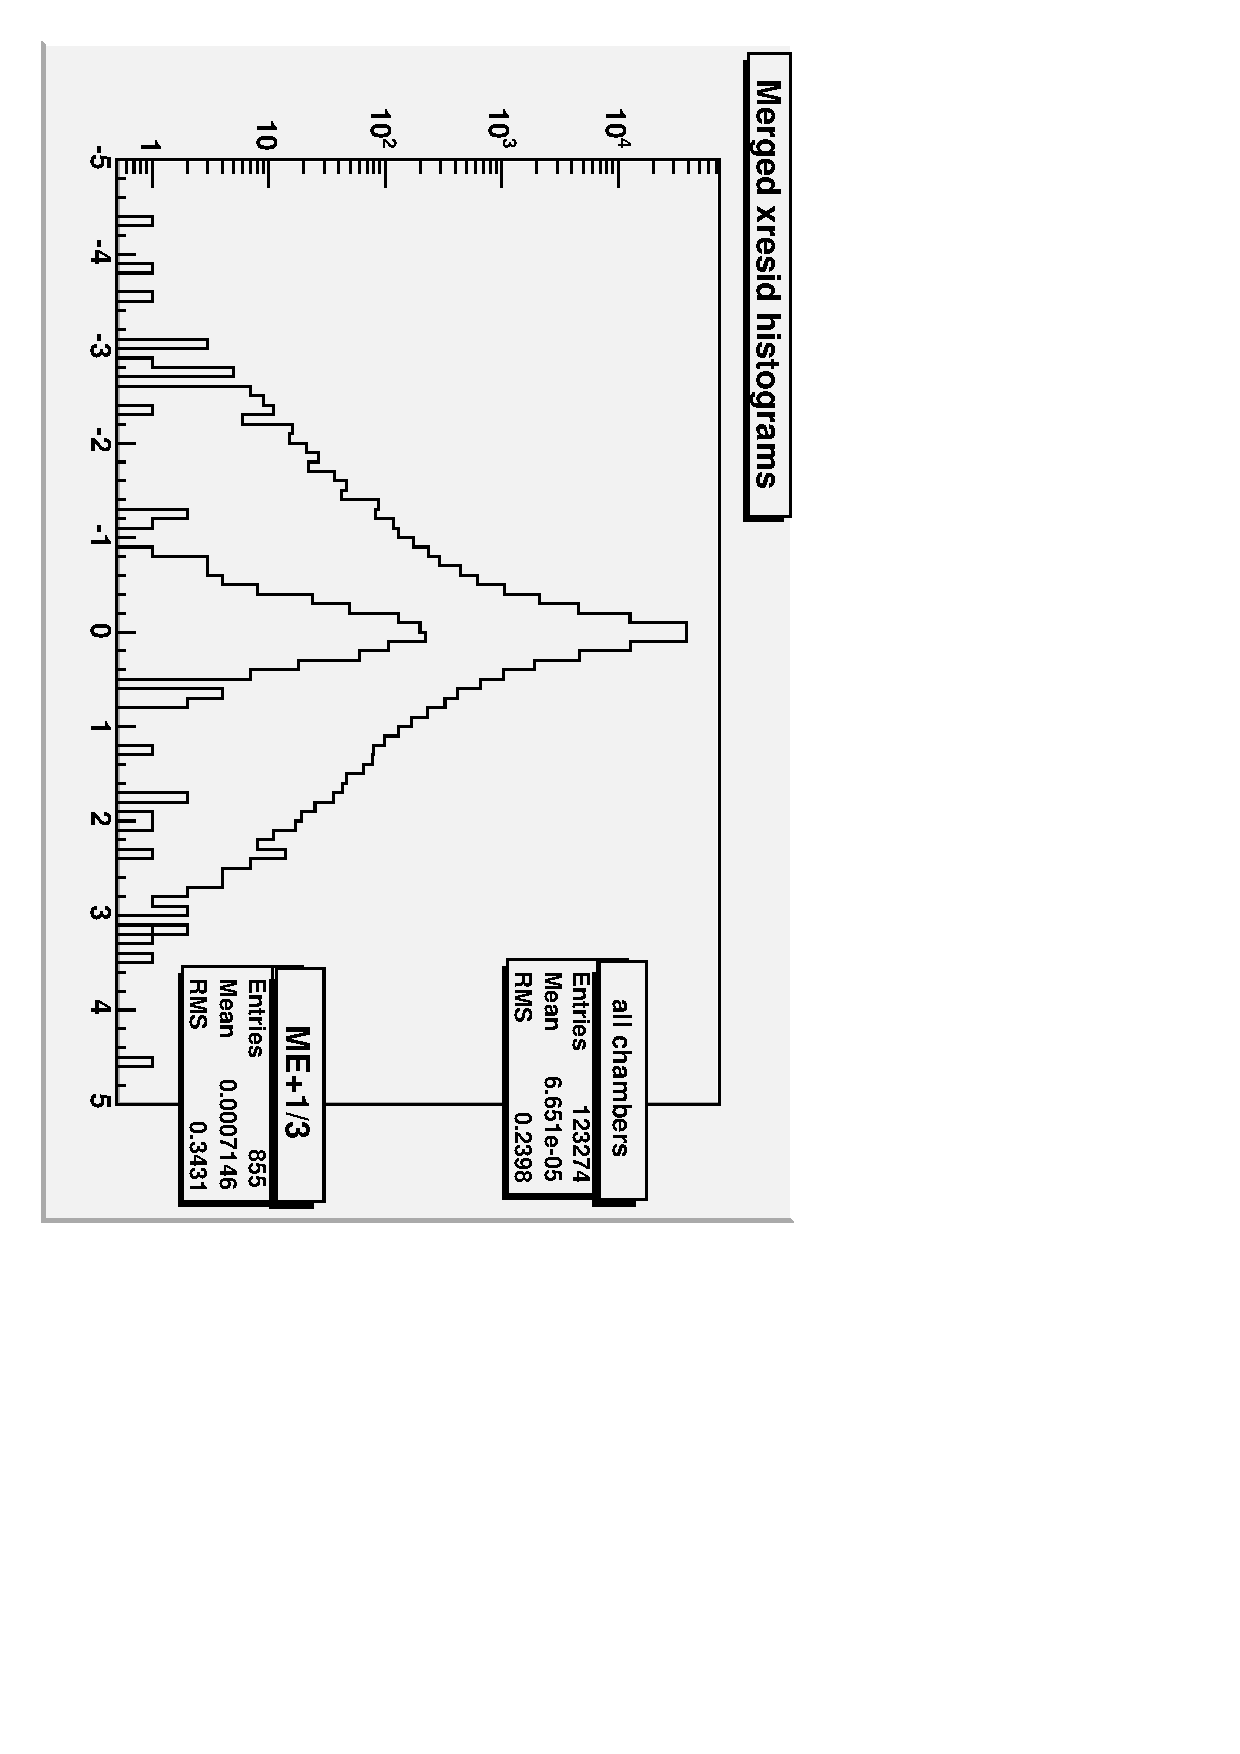
\includegraphics[height=\linewidth, angle=90]{affected_chambers_xresid.pdf}
\end{minipage}
\end{tabular}
\end{center}
\end{frame}

\begin{frame}
\frametitle{Update: intrinsic resolutions in MTCC}

\begin{center}
\begin{tabular}{p{0.4\linewidth} c p{0.4\linewidth}}
  \begin{minipage}{\linewidth}
    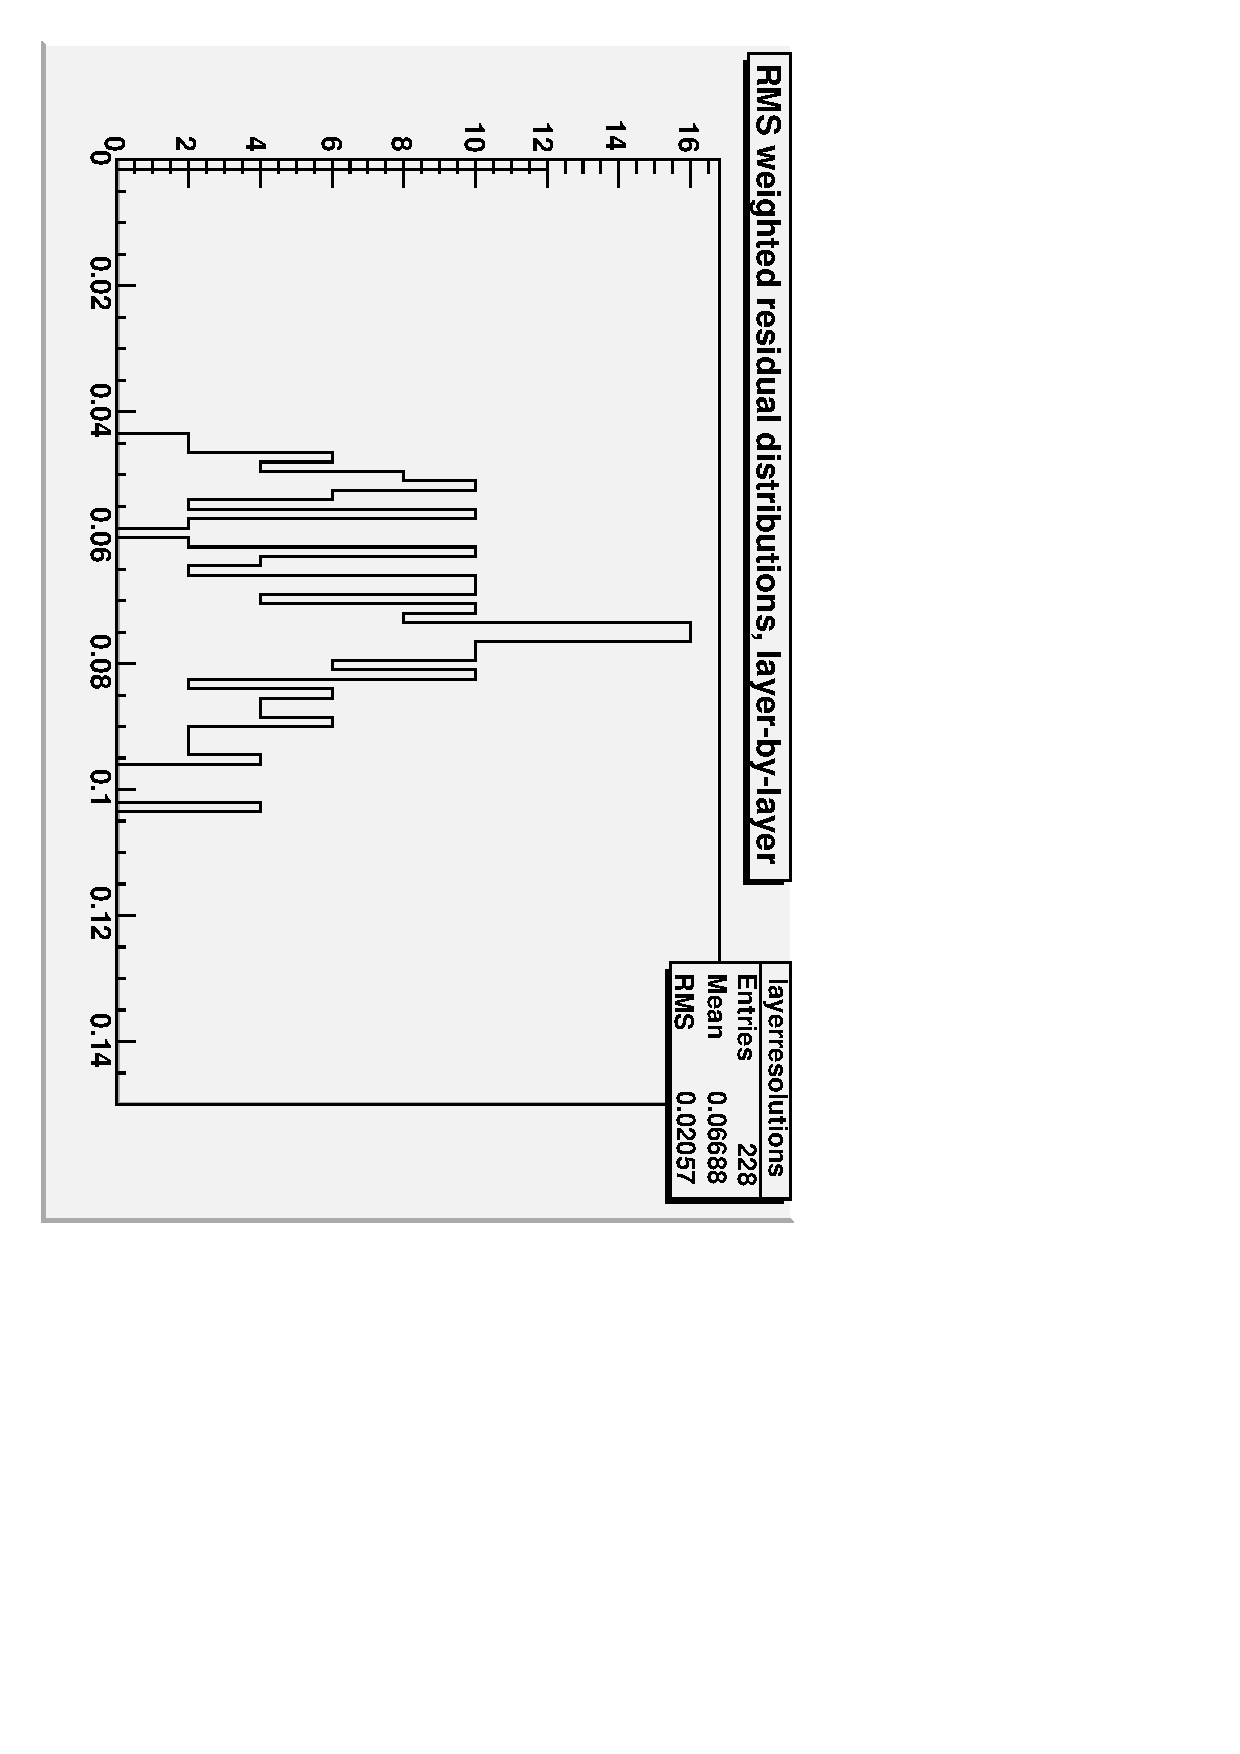
\includegraphics[height=\linewidth, angle=90]{rms_of_layer_distributions.pdf}
  \end{minipage} & &
  \begin{minipage}{\linewidth}
    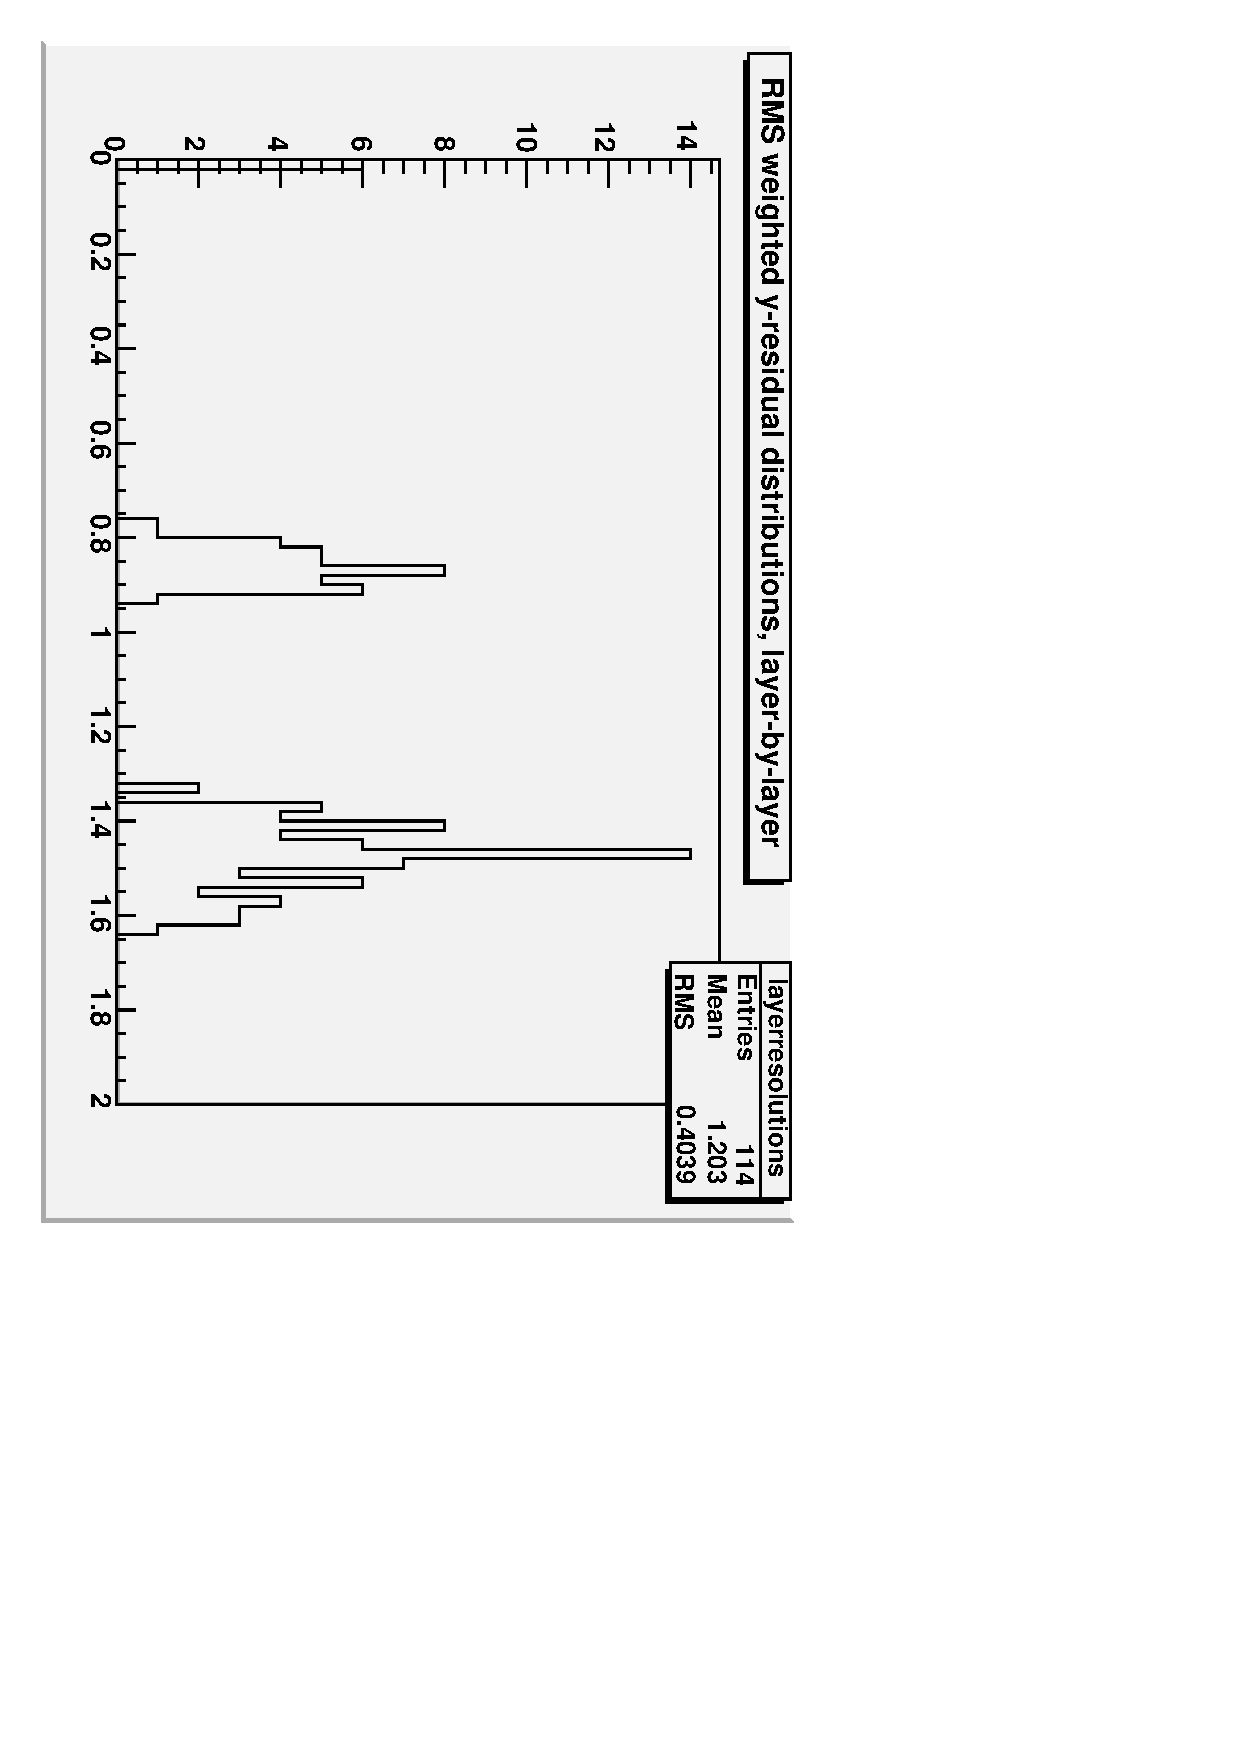
\includegraphics[height=\linewidth, angle=90]{rms_of_layer_yresid_distributions.pdf}
  \end{minipage} \\
  & & \\
  \begin{minipage}{\linewidth}
    \begin{center}
      RMS of layer weighted $x$ residual distributions
    \end{center}
  \end{minipage} & &
  \begin{minipage}{\linewidth}
    \begin{center}
      RMS of layer weighted $y$ residual distributions
    \end{center}
  \end{minipage} \\
\end{tabular}
\end{center}

\vfill $x$ residual RMS of 400 $\mu$m to 1 mm

\vfill Clear distinction between broad and narrow $y$ residual distributions
\end{frame}

\begin{frame}
\frametitle{Short-term plans}
\begin{itemize}\setlength{\itemsep}{0.25 cm}
\item MC tests:

\begin{itemize}
\item Align muon system to tracker: globalMuons with deweighted muon system (running)

\item Align muon system to itself: fit standAloneMuons to
  even-numbered stations, align odd, alternate

\item Layer-by-layer alignments should not suffer from tracking bias
  due to ``smoothed residuals,'' so align with no deweighting (running)

\item ``New feature deadline'' for CSA07 is next Wednesday!  Deweighting is a new feature!
\end{itemize}

\item MTCC analysis:

\begin{itemize}
\item Try a simple layer-by-layer alignment

\item Try even/odd chamber-by-chamber alignment

\item Compare AlignmentProducer results with ToyAlignment? (Non-trivial due to different constraints\ldots)

\end{itemize}
\end{itemize}
\label{numpages}
\end{frame}

\end{document}
